\chapter{Evaluation of the \textit{i}MGXS Scheme}
\label{chap:results}

The preceding chapter introduced a methodology for \textit{inferential multi-group cross section} (\textit{i}\ac{MGXS}) spatial homogenization. The \textit{i}\ac{MGXS} scheme uses unsupervised clustering algorithms to infer the optimal assignment of fuel pin instances to spatial homogenization tally zones based on an analysis of ``noisy'' \ac{MC} tally data. This chapter evaluates \textit{i}\ac{MGXS} homogenization with respect to the scheme's two primary objectives:

\begin{itemize}[noitemsep]
\item Approach the \textbf{accuracy} of \textit{degenerate} spatial homogenization (Sec.~\ref{subsec:chap8-degenerate})
\item Approach the \ac{MC} \textbf{convergence} of \textit{null} spatial homogenization (Sec.~\ref{subsec:chap8-null})
\end{itemize}

\noindent Furthermore, the \textit{i}\ac{MGXS} scheme seeks to address the shortcomings of the Local Neighbor Symmetry (\ac{LNS}) spatial homogenization scheme (Sec.~\ref{sec:chap9-lns-homogenize}) -- namely, its inability to flexibly distinguish \ac{MGXS} clusters in arbitrary geometries (\textit{e.g.}, pins along assembly-assembly and assembly-reflector interfaces) and its poor scalability for large geometries -- and represent a pathway for reactor agnostic \ac{MGXS} generation.

The results presented in this chapter reflect the key observations made in Chaps.~\ref{chap:quantify} and~\ref{chap:spatial} for the null, degenerate and \ac{LNS} homogenization schemes. First, it was observed that pin-wise homogenization with track density-weighted \ac{MGXS} (Sec.~\ref{subsec:chap8-fiss-rates}) has no impact on the resultant eigenvalue since all schemes preserve global reactivity. In addition, it was shown that pin-wise \ac{MGXS} clustering must be accounted for to accurately predict pin-wise U-238 capture rates, but it is much less consequential for accurate fission rate predictions. These results inform the results and analysis presented in this chapter.

The accuracy of the \textit{i}\ac{MGXS} scheme is evaluated with respect to the null and degenerate schemes in Sec.~\ref{subsec:chap11-imgxs-results}. The analysis includes a presentation of the eigenvalue bias and the distributions of pin-wise U-238 capture rate errors for four clustering algorithms (Sec.~\ref{sec:chap10-train-predictor}) with varying numbers of clusters, for each of the six heterogeneous \ac{PWR} benchmarks (Sec.~\ref{sec:chap7-benchmarks}). The convergence rate of the OpenMOC solutions with the null, degenerate and \textit{i}\ac{MGXS} schemes is presented in Sec.~\ref{sec:chap11-converge} for ``noisy'' \ac{MC} tally data computed with varying numbers of particle histories. Sec.~\ref{sec:chap11-model-select} examines the empirical results for model selection criteria (Sec.~\ref{sec:chap10-model-select}) which may be use to select the most appropriate number of clusters for the \textit{i}\ac{MGXS} scheme. Finally, Sec.~\ref{sec:chap11-synthesis} concludes with an analysis of the computational resource requirements necessary to reach a desired level of accuracy for pin-wise U-238 capture rates for a reference \ac{MC} calculation in comparison to deterministic multi-group calculations with the degenerate and \textit{i}\ac{MGXS} schemes.


%%%%%%%%%%%%%%%%%%%%%%%%%%%%%%%%%%%%%%%%%%%%%%%%%%%%%%%%%%%%%%%%%%%%%%%%%%%%%%%%
\section{Multi-Group Results with \textit{i}MGXS}
\label{subsec:chap11-imgxs-results}

The \texttt{openmc.mgxs} module (Sec.~\ref{subsec:chap4-mgxs}) was used to compute 70-group \ac{MGXS} with OpenMC, along with all other tallies necessary to compute each of the features described in Sec.~\ref{sec:chap10-feature-extract}. In contrast to the \ac{MGXS} generated with OpenMC in Chaps.~\Crefrange{chap:quantify}{chap:unsupervised}, the \ac{MGXS} used in this chapter were generated with 10$\times$ more batches and 10$\times$ fewer histories per batch. The use of so many active batches made it possible to evaluate the convergence rate of the OpenMOC solutions in Sec.~\ref{sec:chap11-converge}\footnote{As a result of the different OpenMC runtime parameters used in this chapter, the OpenMOC eigenvalues and capture rate errors differ slightly from those reported in Chaps.~\Crefrange{chap:quantify}{chap:unsupervised}. The preceding chapters use 8 -- 9 $\times$ 10$^{8}$ active histories to generate \ac{MGXS}, while this chapter use 9.8 -- 9.9 $\times$ 10$^{8}$ active histories, since fewer histories are expended in the inactive cycles. Although so few histories per batch might risk under-sampling of the fission source distribution for a reference \ac{MC} calculation, it is less of a concern here since it is assumed that under-sampling is not as problematic for \ac{MGXS} generation.}. In particular, the OpenMC simulations were performed with 10,000 batches of 10$^{5}$ particle histories per batch for the assembly and colorset benchmarks, while 10$^{6}$ histories per batch were used for the quarter core \ac{BEAVRS} model. Stationarity of the fission source was obtained with 200 inactive batches for the \ac{BEAVRS} model, while 100 inactive batches were employed for the other five benchmarks (Sec.~\ref{subsec:chap7-src-stationarity}). OpenMC's ``iso-in-lab'' feature (Sec.~\ref{subsec:chap4-iso-in-lab}) was employed to enable consistent comparisons between OpenMC's reference results and OpenMOC's calculations with an isotropic in lab scattering source.

%-how many batches for full core??

The 70-group \ac{MC} tally data was condensed to 2-groups for feature extraction within the \textit{i}\ac{MGXS} data processing pipeline. The litmus-only feature selection approach used the reaction fraction thresholding litmus test (Sec.~\ref{subsubsec:chap10-litmus-react-frac}) to select the ``best'' reaction type for each pair of nuclides and energy groups, for each nuclide in the fuel and both energy groups. All available features were used for each selected reaction type, nuclide and energy group. No dimensionality reduction techniques (Sec.~\ref{sec:chap10-dimension-reduce}) were applied to the selected features. The $k$-means, agglomerative, BIRCH and Gaussian Mixture Model (GMM) clustering algorithms were separately used to train predictors for varying numbers of clusters (Sec.~\ref{sec:chap10-train-predictor}) to inform pin-wise spatial homogenization.

Each of the six benchmarks was modeled with OpenMOC using \ac{MGXS} generated by the \textit{i}\ac{MGXS} spatial homogenization scheme with the same runtime parameters as those used in Chap.~\ref{chap:quantify} for infinite, null and degenerate homogenization, and in Chap.~\ref{chap:spatial} for \ac{LNS} homogenization. The eigenvalue bias is presented in Sec.~\ref{subsec:chap11-imgxs-eigenvalues}, while the U-238 capture rate errors are analyzed in Sec.~\ref{subsec:chap11-imgxs-capt-rates}. The pin-wise fission rate errors for the \textit{i}\ac{MGXS} scheme are not considered here since \ac{MGXS} clustering was previously shown to be largely inconsequential for fission rate predictions.

%%%%%%%%%%%%%%%%%%%%%%%%
\subsection{Eigenvalues}
\label{subsec:chap11-imgxs-eigenvalues}

The OpenMOC eigenvalues were compared to the reference OpenMC eigenvalues from Tab.~\ref{table:chap7-ref-eigenvalues}. The eigenvalue bias $\Delta\rho$ was computed from Eqn.~\ref{eqn:chap5-delta-rho} in units of \ac{pcm}. The bias is listed in Tab.~\ref{table:chap11-eigenvalues} for each benchmark, and varying numbers of clusters for each clustering algorithm. The same trends highlighted in Sec.~\ref{subsec:chap8-eigenvalues} observed from the null and degenerate biases in Tab.~\ref{table:chap8-openmoc-eigenvalues} remain true for \textit{i}\ac{MGXS} spatial homogenization. The \textit{i}\ac{MGXS} eigenvalues are within 10 \ac{pcm} of those computed with both null and degenerate homogenization for all benchmarks. As previously noted in Sec.~\ref{subsec:chap8-eigenvalues}, this is expected since the \ac{MGXS} for the null, degenerate and \textit{i}\ac{MGXS} schemes are homogenized from the same flux and should preserve globally-integrated reaction rates. Hence, neither the type of clustering algorithm nor the number of clusters is expected to systematically impact OpenMOC's eigenvalue predictions. Nevertheless, the consistent eigenvalue biases do support the conclusion that the \textit{i}\ac{MGXS} scheme is properly implemented.

\begin{table}[ht!]
  \centering
  \caption[Eigenvalue bias with \textit{i}MGXS homogenization]{OpenMOC eigenvalue bias $\Delta\rho$ for \textit{i}\ac{MGXS} spatial homogenization.}
  \small
  \label{table:chap11-eigenvalues}
  \vspace{6pt}
  \begin{tabular}{l l R{1.2cm} R{1.2cm} R{1.2cm} R{1.2cm} R{1.2cm} R{1.2cm}}
  \toprule
  \rowcolor{lightgray}
  & \multicolumn{1}{c}{\cellcolor{lightgray} \bf Clustering} & \multicolumn{6}{S[table-format=6.1]}{\cellcolor{lightgray} \textbf{\# Clusters}} \\
  \multirow{-2}{*}{\cellcolor{lightgray} \bf Benchmark} &
  \multicolumn{1}{c}{\cellcolor{lightgray} \bf Algorithm} &
%  \multicolumn{1}{c}{\cellcolor{lightgray} \bf 1\footnotemark} &
  \multicolumn{1}{c}{\cellcolor{lightgray} \bf Null} &
  \multicolumn{1}{c}{\cellcolor{lightgray} \bf 2} &
  \multicolumn{1}{c}{\cellcolor{lightgray} \bf 4} &
  \multicolumn{1}{c}{\cellcolor{lightgray} \bf 8} &
  \multicolumn{1}{c}{\cellcolor{lightgray} \bf 16} &
%  \multicolumn{1}{c}{\cellcolor{lightgray} \bf \# pins\footnotemark} \\
  \multicolumn{1}{c}{\cellcolor{lightgray} \bf Degenerate} \\
  \midrule
\multirow{4}{*}{\parbox{2.5cm}{1.6\% Assm}} & Agglomerative & \multirow{4}{*}{-168} & -168 & -168 & -168 & -168 & \multirow{4}{*}{-168} \\
& BIRCH & & -168 & -168 & -168 & -168 & \\
& \ac{GMM} & & -168 & -168 & -168 & -168 & \\
& $k$-means & & -168 & -168 & -168 & -168 & \\
  \midrule
\multirow{4}{*}{\parbox{2.5cm}{3.1\% Assm}} & Agglomerative & \multirow{4}{*}{-194} & -194 & -194 & -194 & -194 & \multirow{4}{*}{-194} \\
& BIRCH & & -194 & -194 & -194 & -194 & \\
& \ac{GMM} & & -194 & -194 & -194 & -194 & \\
& $k$-means & & -194 & -194 & -194 & -194 & \\
  \midrule
\multirow{4}{*}{\parbox{2.5cm}{3.1\% Assm w/ 20 \acp{BP}}} & Agglomerative & \multirow{4}{*}{-240} & -237 & -236 & -235 & -235 & \multirow{4}{*}{-235} \\
& BIRCH & & -237 & -236 & -235 & -235 & \\
& \ac{GMM} & & -236 & -235 & -236 & -235 & \\
& $k$-means & & -236 & -236 & -236 & -235 & \\
  \midrule
\multirow{4}{*}{\parbox{2.5cm}{2$\times$2 Colorset}} & Agglomerative & \multirow{4}{*}{-191} & -189 & -189 & -189 & -189 & \multirow{4}{*}{-188} \\
& BIRCH & & -189 & -189 & -189 & -188 & \\
& \ac{GMM} & & -188 & -189 & -188 & -189 &  \\
& $k$-means & & -188 & -189 & -188 & -189 & \\
  \midrule
\multirow{4}{*}{\parbox{2.5cm}{2$\times$2 Colorset w/ Reflector}} & Agglomerative & \multirow{4}{*}{-141} & -136 & -136 & -134 & -129 & \multirow{4}{*}{-141} \\
& BIRCH & & -138 & -137 & -136 & -132 & \\
& \ac{GMM} & & -136 & -136 & -137 & -132 & \\
& $k$-means & & -136 & -136 & -134 & -132 & \\
  \midrule
\multirow{4}{*}{\parbox{2.5cm}{BEAVRS Quarter Core}} & Agglomerative & \multirow{4}{*}{-122} & -115 & -117 & -117 & -117 & \multirow{4}{*}{-116} \\
& BIRCH & & -115 & -116 & -115 & -117 & \\
& \ac{GMM} & & -120 & -116 & -116 & -117 & \\
& $k$-means & & -118 & -115 & -117 & -117 & \\
  \bottomrule
\end{tabular}
\end{table}

\addtocounter{footnote}{-2}
\stepcounter{footnote}
\footnotetext{\label{null}Null homogenization is equivalent to \textit{i}\ac{MGXS} homogenization with a single cluster.}

\stepcounter{footnote}
\footnotetext{\label{degenerate}Degenerate homogenization is equivalent to \textit{i}\ac{MGXS} homogenization with a cluster for each fuel pin.}

\vspace{-0.05in}

\begin{emphbox}
\textbf{The OpenMOC eigenvalues for \textit{i}\ac{MGXS} homogenization are consistent to within 10 \ac{pcm}  for all numbers of clusters due to the preservation of global reactivity.}
\end{emphbox}

%%%%%%%%%%%%%%%%%%%%%%%%%%%%%%%%
\subsection{U-238 Capture Rates}
\label{subsec:chap11-imgxs-capt-rates}

The OpenMOC energy-integrated pin-wise U-238 capture rates were compared to the reference OpenMC capture rates for \textit{i}\ac{MGXS} homogenization to compute the percent relative errors for each pin's capture rates. Sec.~\ref{subsec:chap11-imgxs-capt-rates-num-clusters} investigates the dependence of the maximum and mean errors with the number of clusters, while Sec.~\ref{subsec:chap11-imgxs-capt-rates-benchmark} compares the errors between null, degenerate and \textit{i}\ac{MGXS} homogenization. Sec.~\ref{subsec:chap11-imgxs-capt-rates-space-distrib} illustrates the spatial distributions of U-238 capture rate errors. Finally, Sec.~\ref{subsec:chap11-imgxs-capt-rates-compare} compares OpenMOC's U-238 capture rate predictions for different clustering models to understand the relative impact of clustered \ac{MGXS} for different types of fuel pins.

%%%%%%%%%%%%%%%%%%%%%%%%%%%%%%%%%%%%%%%%%%%%%%%%%%%%%
\subsubsection{Variation with the Number of Clusters}
\label{subsec:chap11-imgxs-capt-rates-num-clusters}

This section compares the U-238 capture rate for each of the four clustering algorithms as the number of clusters is varied. The simplest clustering model assigns all fuel pin instances to the same cluster, which is equivalent to null homogenization; conversely, the most complex clustering model assigns each fuel pin instance to its own unique cluster, which is equivalent to degenerate homogenization. Based on the results for \ac{LNS} homogenization, it is expected that the U-238 capture rate error can approach that of degenerate homogenization with only perhaps 10 -- 20 clusters for the assembly and colorset benchmarks. Beyond this point, it is expected that there are diminishing returns to increased model complexity. 

\begin{figure}[ht!]
\centering
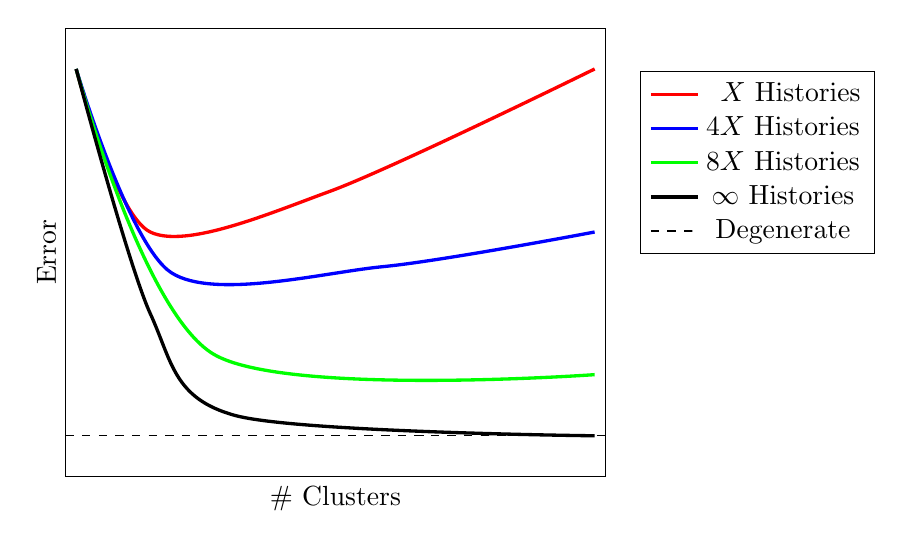
\begin{tikzpicture}
\begin{axis}[xmin=0,xmax=51,ymin=0,ymax=1.1,xlabel={\# Clusters},ylabel={Error},xticklabels={},yticklabels={},xtick={},ytick={},ticks=none,legend style={at={(1.5,0.7)},anchor=east,legend columns=1}]
\addplot[smooth,red,very thick] coordinates { (1,1) (8,0.6) (25,0.7) (50,1) };
\addplot[smooth,blue,very thick] coordinates { (1,1) (10,0.5) (30,0.515) (50,0.6) };
\addplot[smooth,green,very thick] coordinates { (1,1) (14,0.3) (50,0.25) };
\addplot[smooth,very thick] coordinates { (1,1) (8,0.4) (16,0.15) (50,0.1) };
\addplot[smooth,dashed] coordinates { (0,0.1) (51,0.1) };
\addlegendentry{$\;\;X$ Histories}
\addlegendentry{$4X$ Histories}
\addlegendentry{$8X$ Histories}
\addlegendentry{$\infty$ Histories}
\addlegendentry{Degenerate}
\end{axis}
\end{tikzpicture}
\caption[Characteristics of reaction rate error convergence]{Characteristics of reaction rate error convergence with \textit{i}\ac{MGXS} in the limit of infinite particle histories to degenerate homogenization with fully converged \ac{MGXS}.}
\label{fig:chap11-coverge-complexity}
\end{figure}

Furthermore, the balance between model complexity and accuracy will depend on the degree of statistical uncertainty present in the \ac{MC} tally data, as depicted in Fig.~\ref{fig:chap11-coverge-complexity}. In particular, the statistical uncertainties of the ``noisy'' \ac{MC} tally data for $X$ particle histories may preclude the \textit{i}\ac{MGXS} scheme from achieving the asymptotic accuracy of the degenerate scheme with fully converged \ac{MGXS}. The inclusion of more clusters in \textit{i}\ac{MGXS} scheme will enable it to approach the asymptotic accuracy of the degenerate scheme if enough particle histories have been simulated to reliably estimate the mean of each \ac{MGXS} cluster. The optimal balance between accuracy and speed is achieved when the majority of the gap in accuracy between the null and degenerate schemes is eliminated with only a few clusters in \textit{i}\ac{MGXS}, which quickly converge with only a fraction of the particle histories needed to converge the \ac{MGXS} for the degenerate scheme.

The maximum and mean errors for \textit{i}\ac{MGXS} with 1 -- 50 clusters are illustrated in Figs.~\Crefrange{fig:chap11-capt-err-by-cluster-assm-16}{fig:capt-err-by-cluster-full-core} for the individual assembly, 2$\times$2 colorset and quarter core \ac{BEAVRS} benchmark models. In particular, the maximum errors are the maximum of the absolute values of the errors, while the mean errors are the averages of the absolute error magnitudes. A couple of key observations can be made with regards to the errors' dependence on the number of clusters, as well as the clustering algorithm. First, it is clear from Figs.~\Crefrange{fig:chap11-capt-err-by-cluster-assm-16}{fig:chap11-capt-err-by-cluster-assm-31-20BPs} that the errors for the individual assemblies is greatly reduced with only 4 -- 8 clusters, with additional clusters having a marginal impact. As expected, the introduction of spatial heterogeneities requires more clusters to converge the error reduction. For example, both the max and mean errors are still trending downward even with 20 clusters for the 2$\times$2 colorset with a water reflector.

%1) the majority of the reduction comes with the inclusion of just a few clusters
%   -max err. for 1.6\% assm (1.1\%) eventually reduces to 0.45\%
%   -just 3 clusters gets to 0.55\%, or 85\% of the reduction with just three clusters
%2) more clusters needed as geometric complexities are added
%   -add BPs
%     -roughly 6 clusters needed for 3.1\% assm, while 10 or so needed with \acp{BP}
%   -add reflector
%     -perioridic colorset mean err saturated with 10 clusters

The different clustering algorithms also vary in terms of their impact on the max and mean error. However, the figures do not clearly indicate which if any of the algorithms consistently under or over-performs the others for all benchmarks. All four algorithms perform similarly for the 1.6\% and 3.1\% enriched fuel assemblies without \acp{BP} for 1 -- 20 clusters, as shown in Figs.~\Crefrange{fig:chap11-capt-err-by-cluster-assm-16}{fig:chap11-capt-err-by-cluster-assm-31}. Although the mean errors are similar for up to 50 clusters for both assemblies, the max errors fluctuate somewhat erratically between 0.2 -- 0.4\% for 20 -- 50 clusters. Similarly, the mean errors for the 3.1\% enriched assembly with 20 \acp{BP} and the 2$\times$2 colorsets exhibit a consistent downward trend, while the maximum errors separate and fluctuate wildly beyond 10 clusters for the four clustering algorithms. Although no algorithm can be clearly chosen as a ``winner,'' the \ac{GMM} algorithm seems to most consistently outperform the other clustering algorithms for 10 or more clusters. 

Finally, it should be noted that while the mean error is generally a smooth, monotonically decreasing curve, the max error exhibits sharp discontinuities with the addition of clusters. The maximum error likely decreases in a step-like fashion when the addition of a new cluster discriminates those fuel pins with the largest error into their own unique cluster. Evidently, new clusters generally do not refine the \ac{MGXS} for pins with the worst errors. This is likely due to the fact that the $k$-means, agglomerative and \ac{GMM} clustering models optimize a global metric representing the cluster assignments of all points in a dataset, rather than the behavior of the most poorly defined cluster in the model. A revised clustering algorithm may be needed to achieve the maximum error reduction with as few clusters as possible, by successively refining the samples in the most poorly defined clusters. The BIRCH algorithm shows some promise with 10 or fewer clusters, which may be the result of its locally optimized assignment of samples to clusters.

\begin{emphbox}
\textbf{Only a few \ac{MGXS} clusters are needed to substantially reduce the U-238 capture rate errors, with diminishing returns for the inclusion of more clusters. None of the clustering algorithms is a clear winner, though BIRCH generally performs the best for <10 clusters, while \acp{GMM} do better with 10+ clusters.}
\end{emphbox}

%-should mention errors with ICA, PCA, or FA to illustrate that clustering can screw up??? 
%-should mention errors look much different for pinch featur selection???

\begin{figure}[h!]
\centering
\begin{subfigure}{0.9\textwidth}
  \centering
  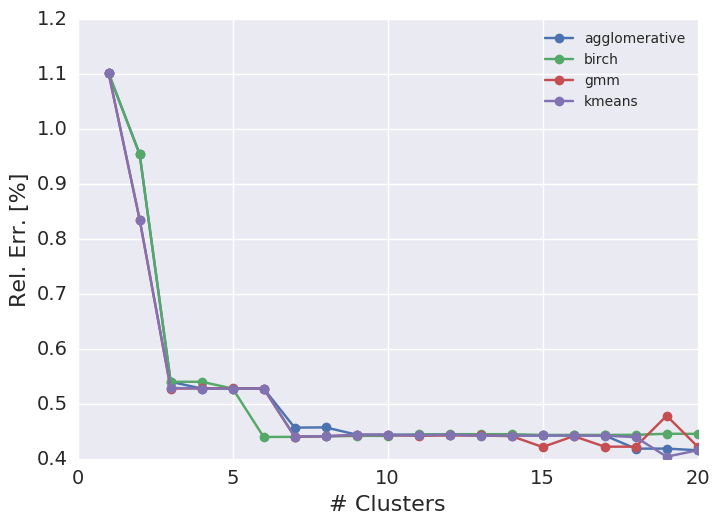
\includegraphics[width=\linewidth]{figures/results/err-by-cluster/assm-16/max-rel-err}
  \caption{}
  \label{fig:chap11-max-capt-err-by-cluster-assm-16}
\end{subfigure}
\begin{subfigure}{0.9\textwidth}
  \centering
  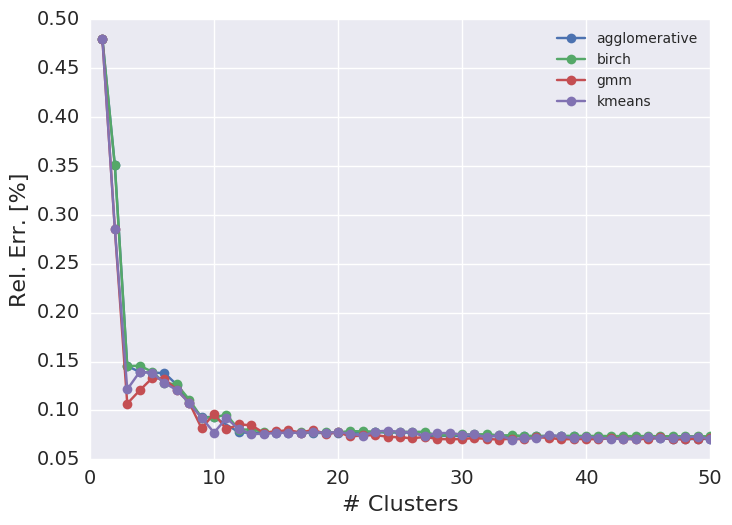
\includegraphics[width=\linewidth]{figures/results/err-by-cluster/assm-16/mean-rel-err}
  \caption{}
  \label{fig:chap11-mean-capt-err-by-cluster-assm-16}
\end{subfigure}
\caption[U-238 capture rate error variation with the number of clusters]{The max (a) and mean (b) U-238 capture rate errors for the 1.6\% enriched assembly with \textit{i}\ac{MGXS} spatial homogenization.}
\label{fig:chap11-capt-err-by-cluster-assm-16}
\end{figure}

\begin{figure}[h!]
\centering
\begin{subfigure}{0.9\textwidth}
  \centering
  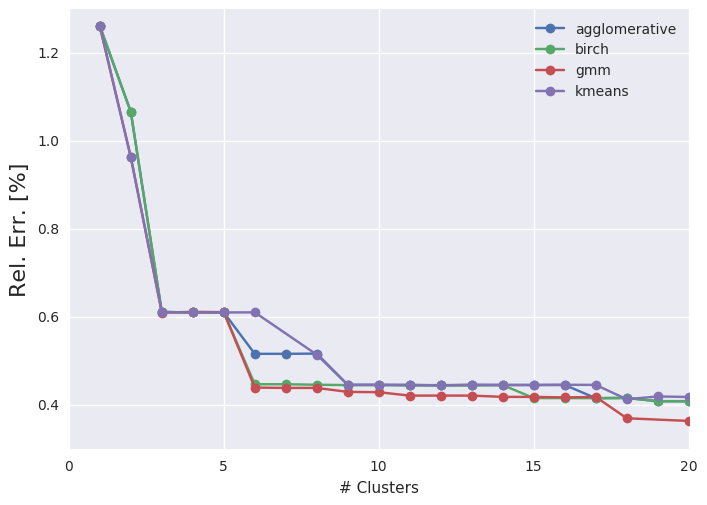
\includegraphics[width=\linewidth]{figures/results/err-by-cluster/assm-31/max-rel-err}
  \caption{}
  \label{fig:chap11-max-capt-err-by-cluster-assm-31}
\end{subfigure}
\begin{subfigure}{0.9\textwidth}
  \centering
  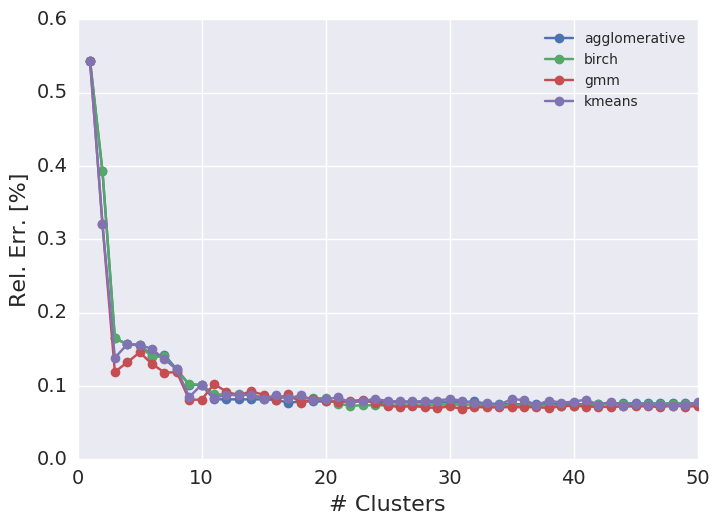
\includegraphics[width=\linewidth]{figures/results/err-by-cluster/assm-31/mean-rel-err}
  \caption{}
  \label{fig:chap11-mean-capt-err-by-cluster-assm-31}
\end{subfigure}
\caption[U-238 capture rate error variation with the number of clusters]{The max (a) and mean (b) U-238 capture rate errors for the 3.1\% enriched assembly with \textit{i}\ac{MGXS} spatial homogenization.}
\label{fig:chap11-capt-err-by-cluster-assm-31}
\end{figure}

\begin{figure}[h!]
\centering
\begin{subfigure}{0.9\textwidth}
  \centering
  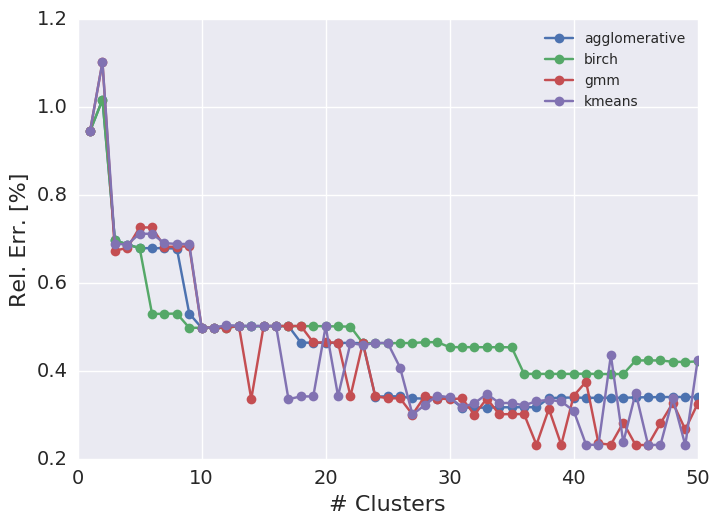
\includegraphics[width=\linewidth]{figures/results/err-by-cluster/assm-31-20BPs/max-rel-err}
  \caption{}
  \label{fig:chap11-max-capt-err-by-cluster-assm-31-20BPs}
\end{subfigure}
\begin{subfigure}{0.9\textwidth}
  \centering
  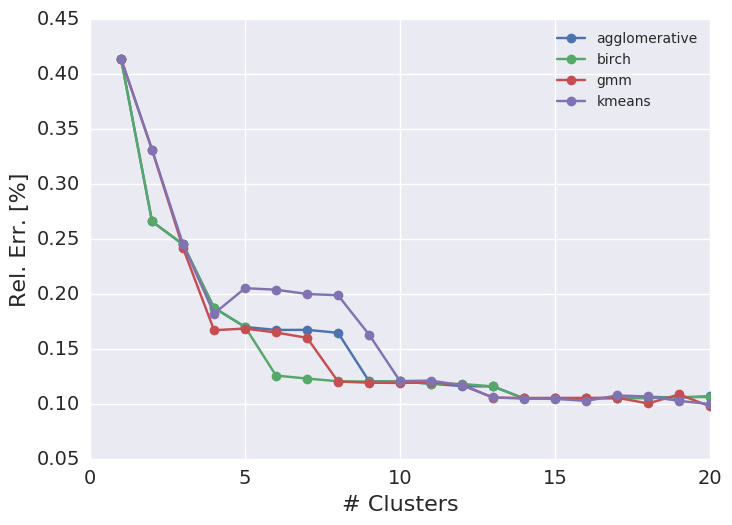
\includegraphics[width=\linewidth]{figures/results/err-by-cluster/assm-31-20BPs/mean-rel-err}
  \caption{}
  \label{fig:chap11-mean-capt-err-by-cluster-assm-31-20BPs}
\end{subfigure}
\caption[U-238 capture rate error variation with the number of clusters]{The max (a) and mean (b) U-238 capture rate errors for the 3.1\% enriched assembly with 20 \acp{BP} with \textit{i}\ac{MGXS} spatial homogenization.}
\label{fig:chap11-capt-err-by-cluster-assm-31-20BPs}
\end{figure}

\begin{figure}[h!]
\centering
\begin{subfigure}{0.9\textwidth}
  \centering
  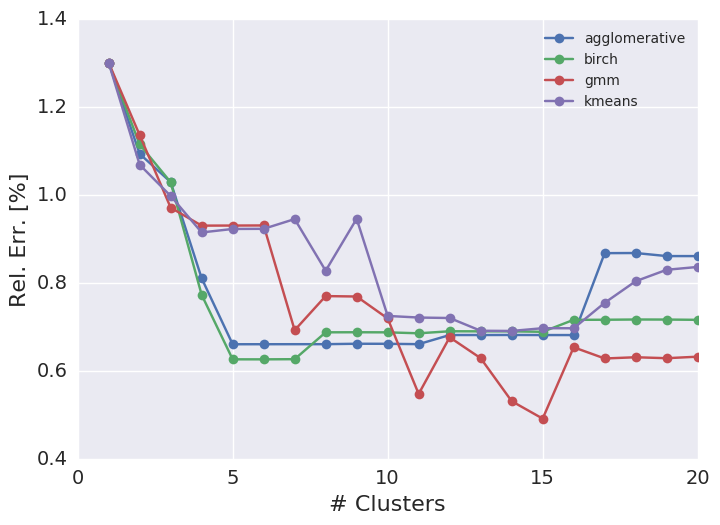
\includegraphics[width=\linewidth]{figures/results/err-by-cluster/2x2/max-rel-err}
  \caption{}
  \label{fig:chap11-max-capt-err-by-cluster-2x2}
\end{subfigure}
\begin{subfigure}{0.9\textwidth}
  \centering
  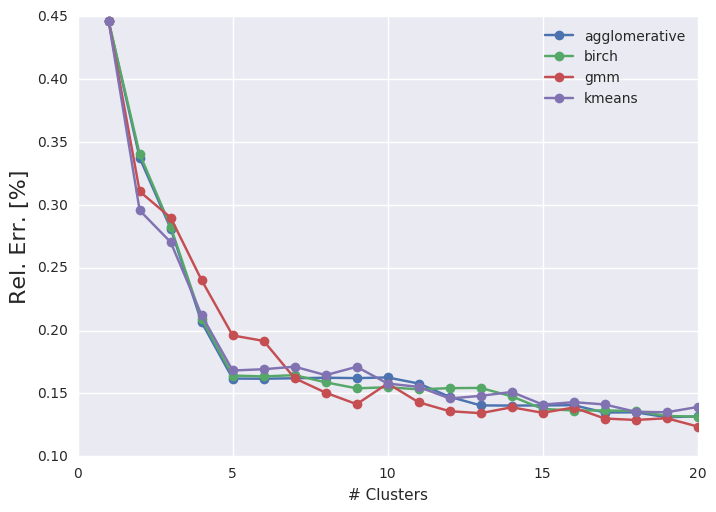
\includegraphics[width=\linewidth]{figures/results/err-by-cluster/2x2/mean-rel-err}
  \caption{}
  \label{fig:chap11-mean-capt-err-by-cluster-2x2}
\end{subfigure}
\caption[U-238 capture rate error variation with the number of clusters]{The max (a) and mean (b) U-238 capture rate error for the 2$\times$2 colorset with \textit{i}\ac{MGXS} spatial homogenization.}
\label{fig:chap11-capt-err-by-cluster-2x2}
\end{figure}

\begin{figure}[h!]
\centering
\begin{subfigure}{0.9\textwidth}
  \centering
  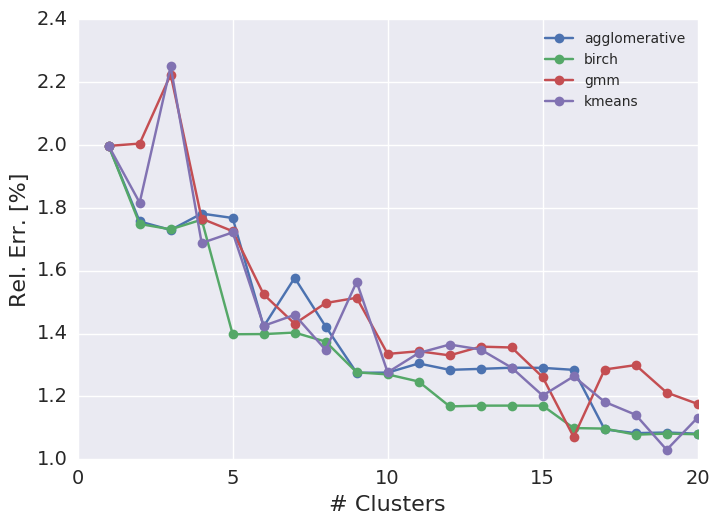
\includegraphics[width=\linewidth]{figures/results/err-by-cluster/reflector/max-rel-err}
  \caption{}
  \label{fig:chap11-max-capt-err-by-cluster-refl}
\end{subfigure}
\begin{subfigure}{0.9\textwidth}
  \centering
  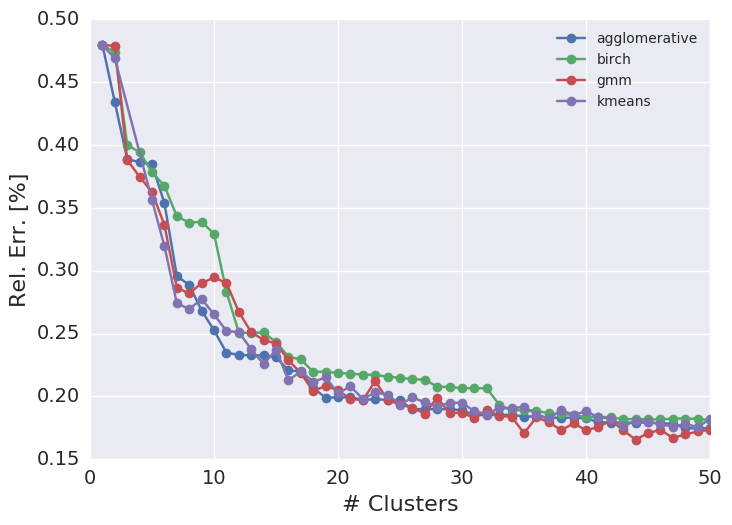
\includegraphics[width=\linewidth]{figures/results/err-by-cluster/reflector/mean-rel-err}
  \caption{}
  \label{fig:chap11-mean-capt-err-by-cluster-refl}
\end{subfigure}
\caption[U-238 capture rate error variation with the number of clusters]{The max (a) and mean (b) U-238 capture rate error for the 2$\times$2 colorset with water reflector with \textit{i}\ac{MGXS} spatial homogenization.}
\label{fig:chap11-capt-err-by-cluster-refl}
\end{figure}

\begin{figure}[h!]
\centering
\begin{subfigure}{0.9\textwidth}
  \centering
  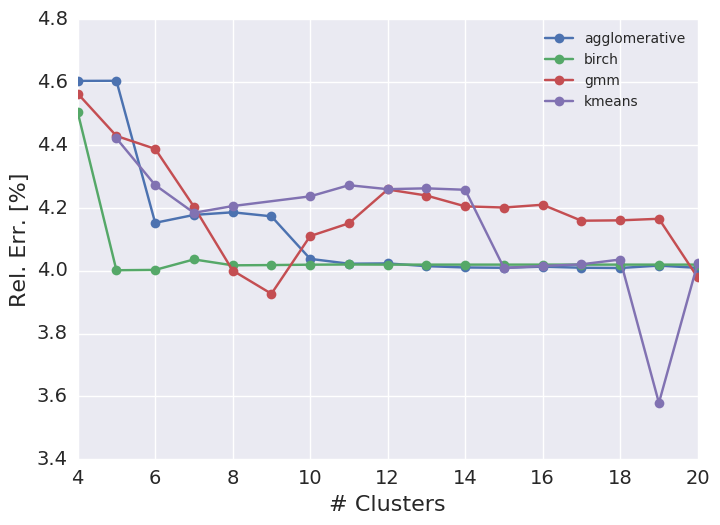
\includegraphics[width=\linewidth]{figures/results/err-by-cluster/full-core/max-rel-err}
  \caption{}
  \label{fig:max-capt-err-by-cluster-full-core}
\end{subfigure}
\begin{subfigure}{0.9\textwidth}
  \centering
  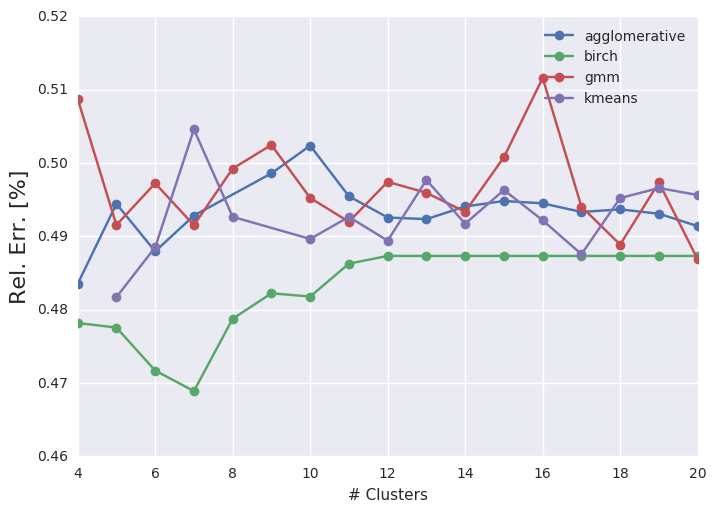
\includegraphics[width=\linewidth]{figures/results/err-by-cluster/full-core/mean-rel-err}
  \caption{}
  \label{fig:mean-capt-err-by-cluster-full-core}
\end{subfigure}
\caption[U-238 capture rate error variation with the number of clusters]{The max (a) and mean (b) U-238 capture rate error for the quarter core \ac{BEAVRS} model with \textit{i}\ac{MGXS} spatial homogenization.}
\label{fig:capt-err-by-cluster-full-core}
\end{figure}

\clearpage

%%%%%%%%%%%%%%%%%%%%%%%%%%%%%%%%%%%%%%%%%%%%%%%%%%%%%%%%%%%%%%
\subsubsection{Benchmark with Null and Degenerate Schemes}
\label{subsec:chap11-imgxs-capt-rates-benchmark}

The maximum and mean percent relative errors for each pin's U-238 capture rates are listed for each benchmark in Tabs.~\ref{table:chap11-max-capt-rates} and~\ref{table:chap11-mean-capt-rates}, respectively, for a variable number of clusters for each clustering algorithm. In particular, the maximum errors are the maximum of the absolute values of the errors along with the appropriate sign, while the mean errors are the averages of the absolute error magnitudes. The errors are tabulated for 2 -- 16 clusters, along with null homogenization (one cluster for all pin instances) and degenerate homogenization (one cluster per pin instance).

Since the tables simply represent a subset of the data illustrated in Figs.~\Crefrange{fig:chap11-capt-err-by-cluster-assm-16}{fig:capt-err-by-cluster-full-core}, the observations made in Sec.~\ref{subsec:chap11-imgxs-capt-rates-num-clusters} remain valid here. First, the majority of the error is reduced with only a few clusters. For example, 70 -- 80\% of the reduction in the maximum error enabled with degenerate homogenization can be achieved with only 4 clusters for the 1.6\% and 3.1\% enriched fuel assembly benchmarks without \acp{BP}. Although 16 clusters (or more) are needed to reduce the error to 70\% for the 3.1\% enriched assembly with 20 \acp{BP}, over 75\% of the error reduction is achieved with only 4 clusters for the periodic 2$\times$2 colorset. Likewise, the addition of a water reflector to the colorset necessitates the use of 16 or more clusters to reduce the error by 75\% or more. In addition, the maximum errors exhibit greater variation across algorithms than the mean errors, as was previously noted in Sec.~\ref{subsec:chap11-imgxs-capt-rates-num-clusters}. Finally, the BIRCH and \ac{GMM} algorithms generally achieve smaller errors than the $k$-means and agglomerative clustering algorithms for a fixed number of clusters.

\begin{table}[h!]
  \centering
  \caption[Maximum U-238 capture rate errors with \textit{i}MGXS homogenization]{Maximum absolute U-238 capture rate percent relative errors for \textit{i}\ac{MGXS} spatial homogenization for each clustering algorithm.}
  \small
  \label{table:chap11-max-capt-rates}
  \vspace{6pt}
  \begin{tabular}{l l R{1.2cm} R{1.2cm} R{1.2cm} R{1.2cm} R{1.2cm} R{1.2cm}}
  \toprule
  \rowcolor{lightgray}
  & \multicolumn{1}{c}{\cellcolor{lightgray} \bf Clustering} & \multicolumn{6}{S[table-format=6.1]}{\cellcolor{lightgray} \textbf{\# Clusters}} \\
  \multirow{-2}{*}{\cellcolor{lightgray} \bf Benchmark} &
  \multicolumn{1}{c}{\cellcolor{lightgray} \bf Algorithm} &
%  \multicolumn{1}{c}{\cellcolor{lightgray} \bf 1\textsuperscript{\ref{null}}} &
  \multicolumn{1}{c}{\cellcolor{lightgray} \bf Null} &
  \multicolumn{1}{c}{\cellcolor{lightgray} \bf 2} &
  \multicolumn{1}{c}{\cellcolor{lightgray} \bf 4} &
  \multicolumn{1}{c}{\cellcolor{lightgray} \bf 8} &
  \multicolumn{1}{c}{\cellcolor{lightgray} \bf 16} &
%  \multicolumn{1}{c}{\cellcolor{lightgray} \bf \# pins\textsuperscript{\ref{degenerate}}} \\
  \multicolumn{1}{c}{\cellcolor{lightgray} \bf Degenerate} \\
  \midrule
\multirow{4}{*}{\parbox{2.5cm}{1.6\% Assm}} & Agglomerative & \multirow{4}{*}{-1.10} & 0.95 & -0.53 & -0.46 & -0.44 & \multirow{4}{*}{0.38} \\
& BIRCH & & 0.95 & -0.54 & -0.44 & -0.44 & \\
& \ac{GMM} & & -0.84 & -0.53 & -0.44 & -0.44 & \\
& $k$-means & & -0.84 & -0.53 & -0.44 & -0.44 & \\
  \midrule
\multirow{4}{*}{\parbox{2.5cm}{3.1\% Assm}} & Agglomerative & \multirow{4}{*}{-1.26} & 1.07 & -0.61 & -0.52 & 0.45 & \multirow{4}{*}{-0.33} \\
& BIRCH & & 1.07 & -0.61 & 0.45 & -0.42 & \\
& \ac{GMM} & & -0.96 & -0.61 & -0.44 & -0.42 & \\
& $k$-means & & -0.96 & -0.61 & -0.52 & 0.45 & \\
  \midrule
\multirow{4}{*}{\parbox{2.5cm}{3.1\% Assm w/ 20 BPs}} & Agglomerative & \multirow{4}{*}{-0.95} & -1.02 & 0.69 & 0.68 & -0.50 & \multirow{4}{*}{-0.30} \\
& BIRCH & & -1.02 & 0.69 & -0.53 & -0.50 & \\
& \ac{GMM} & & -1.10 & 0.68 & -0.53 & -0.50 & \\
& $k$-means & & -1.10 & 0.69 & -0.69 & 0.34 & \\
  \midrule
\multirow{4}{*}{\parbox{2.5cm}{2$\times$2 Colorset}} & Agglomerative & \multirow{4}{*}{-1.30} & -1.09 & 0.81 & 0.66 & 0.68 & \multirow{4}{*}{-0.64} \\
& BIRCH & & -1.12 & 0.77 & 0.69 & 0.72 & \\
& \ac{GMM} & & -1.14 & 0.93 & 0.77 & 0.65 & \\
& $k$-means & & -1.07 & -0.92 & -0.83 & 0.70 & \\
  \midrule
\multirow{4}{*}{\parbox{2.5cm}{2$\times$2 Colorset w/ Reflector}} & Agglomerative & \multirow{4}{*}{-2.00} & -1.76 & -1.78 & -1.42 & -1.28 & \multirow{4}{*}{-0.80} \\
& BIRCH & & -1.75 & -1.76 & -1.37 & 1.10 & \\
& \ac{GMM} & & -2.00 & -1.77 & 1.50 & 1.07 & \\
& $k$-means & & -1.82 & -1.69 & 1.35 & -1.26 & \\
  \midrule
\multirow{4}{*}{\parbox{2.5cm}{BEAVRS Quarter Core}} & Agglomerative & \multirow{4}{*}{-4.78} & -4.36 & -3.51 & -3.44 & -3.43 & \multirow{4}{*}{-3.03} \\
& BIRCH & & -4.44 & -3.37 & -2.60 & -2.27 & \\
& \ac{GMM} & & -4.63 & -3.50 & -3.57 & -3.88 & \\
& $k$-means & & -4.38 & -3.81 & -3.49 & -3.46 & \\
  \bottomrule
\end{tabular}
\end{table}

\clearpage

\begin{table}[h!]
  \centering
  \caption[Mean U-238 capture rate errors with \textit{i}MGXS homogenization]{Mean absolute U-238 capture rate percent relative errors for \textit{i}\ac{MGXS} spatial homogenization for each clustering algorithm.}
  \small
  \label{table:chap11-mean-capt-rates}
  \vspace{6pt}
  \begin{tabular}{l l R{1.2cm} R{1.2cm} R{1.2cm} R{1.2cm} R{1.2cm} R{1.2cm}}
  \toprule
  \rowcolor{lightgray}
  & \multicolumn{1}{c}{\cellcolor{lightgray} \bf Clustering} & \multicolumn{6}{S[table-format=6.1]}{\cellcolor{lightgray} \textbf{\# Clusters}} \\
  \multirow{-2}{*}{\cellcolor{lightgray} \bf Benchmark} &
  \multicolumn{1}{c}{\cellcolor{lightgray} \bf Algorithm} &
%  \multicolumn{1}{c}{\cellcolor{lightgray} \bf 1\textsuperscript{\ref{null}}} &
  \multicolumn{1}{c}{\cellcolor{lightgray} \bf Null} &
  \multicolumn{1}{c}{\cellcolor{lightgray} \bf 2} &
  \multicolumn{1}{c}{\cellcolor{lightgray} \bf 4} &
  \multicolumn{1}{c}{\cellcolor{lightgray} \bf 8} &
  \multicolumn{1}{c}{\cellcolor{lightgray} \bf 16} &
%  \multicolumn{1}{c}{\cellcolor{lightgray} \bf \# pins\textsuperscript{\ref{degenerate}}} \\
  \multicolumn{1}{c}{\cellcolor{lightgray} \bf Degenerate} \\
  \midrule
\multirow{4}{*}{\parbox{2.5cm}{1.6\% Assm}} & Agglomerative & \multirow{4}{*}{0.48} & 0.35 & 0.14 & 0.11 & 0.08 & \multirow{4}{*}{0.08} \\
& BIRCH & & 0.35 & 0.15 & 0.11 & 0.08 & \\
& \ac{GMM} & & 0.29 & 0.12 & 0.11 & 0.08 & \\
& $k$-means & & 0.29 & 0.14 & 0.11 & 0.08 & \\
  \midrule
\multirow{4}{*}{\parbox{2.5cm}{3.1\% Assm}} & Agglomerative & \multirow{4}{*}{0.54} & 0.39 & 0.16 & 0.12 & 0.08 & \multirow{4}{*}{0.09} \\
& BIRCH & & 0.39 & 0.16 & 0.12 & 0.08 \\
& \ac{GMM} & & 0.32 & 0.13 & 0.10 & 0.09 & \\
& $k$-means & & 0.32 & 0.16 & 0.12 & 0.09 & \\
  \midrule
\multirow{4}{*}{\parbox{2.5cm}{3.1\% Assm w/ 20 BPs}} & Agglomerative & \multirow{4}{*}{0.41} & 0.27 & 0.19 & 0.17 & 0.11 & \multirow{4}{*}{0.09} \\
& BIRCH & & 0.27 & 0.19 & 0.12 & 0.11 & \\
& \ac{GMM} & & 0.33 & 0.17 & 0.12 & 0.11 & \\
& $k$-means & & 0.33 & 0.18 & 0.20 & 0.10 & \\
  \midrule
\multirow{4}{*}{\parbox{2.5cm}{2$\times$2 Colorset}} & Agglomerative & \multirow{4}{*}{0.45} & 0.34 & 0.21 & 0.16 & 0.14 & \multirow{4}{*}{0.15} \\
& BIRCH & & 0.34 & 0.21 & 0.16 & 0.14 & \\
& \ac{GMM} & & 0.31 & 0.24 & 0.15 & 0.14 & \\
& $k$-means & & 0.30 & 0.21 & 0.16 & 0.14 & \\
  \midrule
\multirow{4}{*}{\parbox{2.5cm}{2$\times$2 Colorset w/ Reflector}} & Agglomerative & \multirow{4}{*}{0.48} & 0.43 & 0.39 & 0.29 & 0.22 & \multirow{4}{*}{0.16} \\
& BIRCH & & 0.47 & 0.39 & 0.34 & 0.23 & \\
& \ac{GMM} & & 0.48 & 0.37 & 0.29 & 0.24 & \\
& $k$-means & & 0.47 & 0.37 & 0.27 & 0.22 & \\
  \midrule
\multirow{4}{*}{\parbox{2.5cm}{BEAVRS Quarter Core}} & Agglomerative & \multirow{4}{*}{0.49} & 0.54 & 0.42 & 0.40 & 0.36 & \multirow{4}{*}{0.39} \\
& BIRCH & & 0.53 & 0.55 & 0.52 & 0.47 & \\
& \ac{GMM} & & 0.56 & 0.47 & 0.44 & 0.44 & \\
& $k$-means & & 0.53 & 0.48 & 0.43 & 0.43 & \\
  \bottomrule
\end{tabular}
\end{table}

\clearpage

%%%%%%%%%%%%%%%%%%%%%%%%%%%%%%%%%%%%%%%%%%%%%%%%%%%%%%%%%%%%%%%%%%
\subsubsection{Spatial Distributions of U-238 Capture Rate Errors}
\label{subsec:chap11-imgxs-capt-rates-space-distrib}

The spatial distributions of capture rate errors are plotted as heatmaps for the assembly and colorset benchmarks in Figs.~\Crefrange{fig:chap11-assm-1.6-capt-err}{fig:chap11-refl-capt-err} with null, degenerate, \ac{LNS} and \textit{i}\ac{MGXS} homogenization with BIRCH clustering of 2, 4 and 16 clusters. The capture rate errors for the full core are illustrated in Fig.~\ref{fig:chap11-full-core-capt-err-a} for null and degenerate homogenization, and in Fig.~\ref{fig:chap11-full-core-capt-err-b} for \textit{i}\ac{MGXS} homogenization with BIRCH clustering of 4 and 16 clusters.

A couple of key conclusions can be drawn from these results. First, the results from Sec.~\ref{subsec:chap11-imgxs-capt-rates-benchmark} indicated that the errors with \textit{i}\ac{MGXS} homogenization with 16 clusters exceed those for degenerate homogenization for both the 3.1\% enriched fuel assembly with 20 \acp{BP} and the periodic 2$\times$2 colorset. This is revealed in the Figs.~\Crefrange{fig:chap11-assm-3.1-20BPs-capt-err}{fig:chap11-2x2-capt-err} which illustrate a systematic bias which differs from that of the degenerate case. In particular, the pins facially and diagonally adjacent to the central instrument tube exhibit the smallest and largest errors in the assembly with 20 \acp{BP}, respectively. Likewise, the pins between the two rings of \acp{BP} in the 3.1\% enriched fuel assembly exhibit the largest errors for the periodic colorset. These observations are particularly interesting since the \ac{LNS} scheme outperforms \textit{i}\ac{MGXS} for these benchmarks while using substantially fewer materials (9 -- 10 \ac{LNS} materials as compared to 16 \textit{i}\ac{MGXS} materials per assembly). Although \ac{LNS} necessarily discriminates those pins adjacent to the instrument tube and \acp{BP} into unique clusters, the \textit{i}\ac{MGXS} scheme only does so if the feature vectors for those fuel pins are well-separated from those for other fuel pins in feature space.

Unlike the \ac{LNS} scheme, the \textit{i}\ac{MGXS} scheme excels at discriminating pins along assembly-assembly and assembly-reflector interfaces as shown in Figs.~\Crefrange{fig:chap11-2x2-capt-err}{fig:chap11-refl-capt-err}\footnote{However, even with 16 clusters, there are some lingering residual errors for pins along the interfaces between the bottom right assembly and its neighbors.}. This is most obvious for the pins along the assembly-reflector interface which exhibit nearly the same error for both null and \ac{LNS} homogenization. The \textit{i}\ac{MGXS} scheme discriminates these pins into unique clusters such that little if any residual bias is observed with 16 clusters. Indeed, the \textit{i}\ac{MGXS} scheme dedicates unique clusters to those pins along the interfaces \textit{before} discriminating interior pins adjacent to \acp{CRGT} and \acp{BP} into clusters. For this reason, \textit{i}\ac{MGXS} may necessarily need to model more unique materials than \ac{LNS} to achieve the same reduction of the maximum pin-wise error.

Finally, it should be noted that the observations made here are specific to the configuration of the \textit{i}\ac{MGXS} data processing pipeline. As noted in Sec.~\ref{sec:chap10-cluster-geometries}, the choice of features and clustering algorithm has a large impact on the clustering model and the resultant spatial distribution of U-238 capture rate errors. In addition, dimensionality reduction adds another degree of freedom to the types of clustered geometries that may be found with the \textit{i}\ac{MGXS} scheme. Future work should systematically examine the spatial error distributions for different configurations of the \textit{i}\ac{MGXS} data processing pipeline to quantify the ability of each to minimize the error with as few clusters as possible.

%In particular, each of the figures for \textit{i}\ac{MGXS} spatial homogenization corresponds to a prediction by the BIRCH clustering algorithm with litmus-only feature selection. 

\begin{emphbox}
\textbf{The \textit{i}\ac{MGXS} scheme does a better job discriminating fuel pins along assembly-assembly and assembly-reflector interfaces than \ac{LNS}, but requires more unique materials to achieve the same reduction in U-238 capture rate errors.}
\end{emphbox}

%-note that \ac{LNS} did better than degenerate for each benchmark except for reflected colorset

\begin{figure}[h!]
\centering
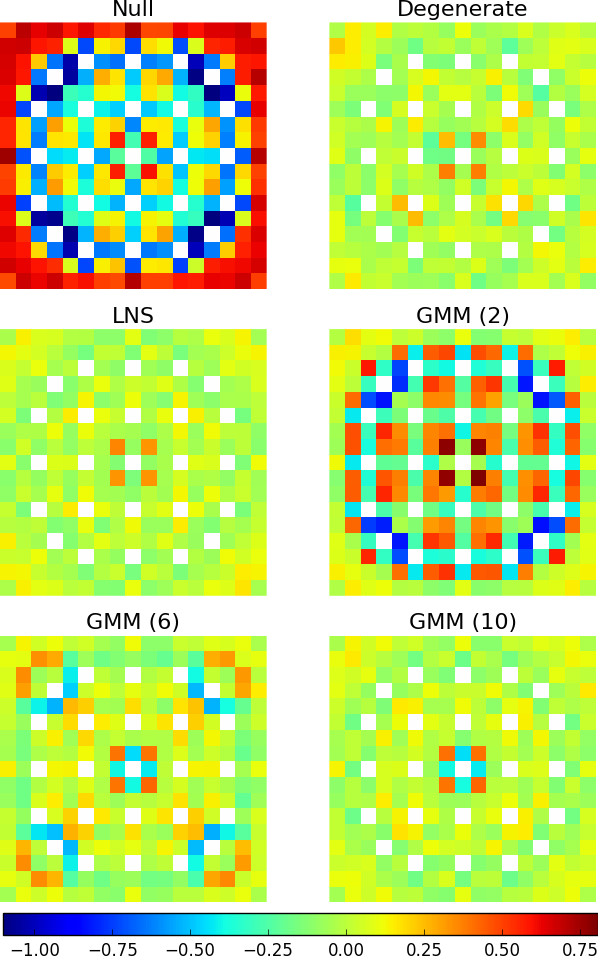
\includegraphics[width=0.87\linewidth]{figures/results/spatial/assm-16/capt-err}
\vspace{2mm}
\caption[U-238 capture rate error spatial distributions]{U-238 capture percent relative errors for the 1.6\% enriched assembly with null, degenerate, \ac{LNS} and \textit{i}\ac{MGXS} spatial homogenization.}
\label{fig:chap11-assm-1.6-capt-err}
\end{figure}

\clearpage

\begin{figure}[h!]
\centering
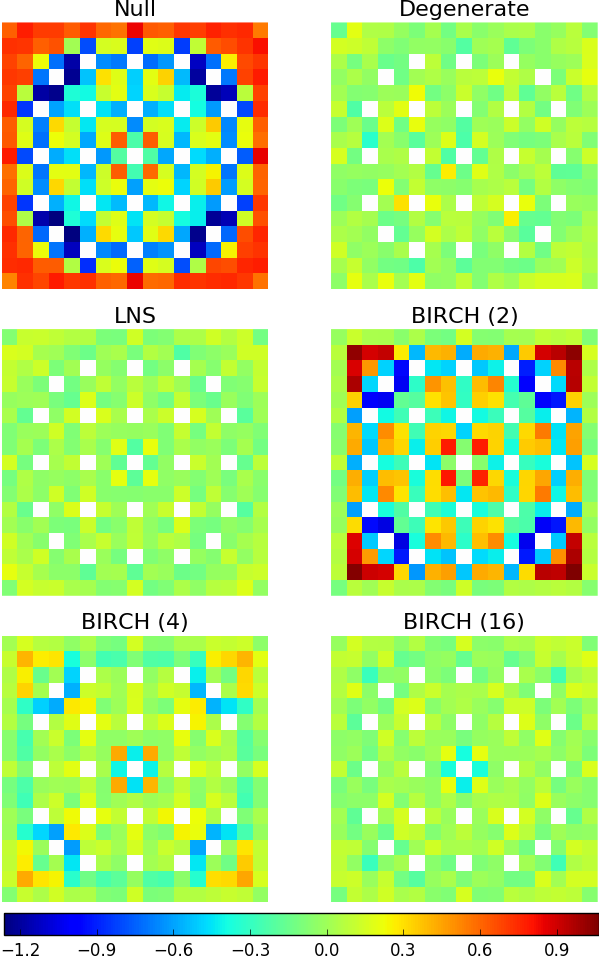
\includegraphics[width=0.87\linewidth]{figures/results/spatial/assm-31/capt-err}
\vspace{2mm}
\caption[U-238 capture rate error spatial distributions]{U-238 capture percent relative errors for the 3.1\% enriched assembly with null, degenerate, \ac{LNS} and \textit{i}\ac{MGXS} spatial homogenization.}
\label{fig:chap11-assm-3.1-capt-err}
\end{figure}

\clearpage

\begin{figure}[h!]
\centering
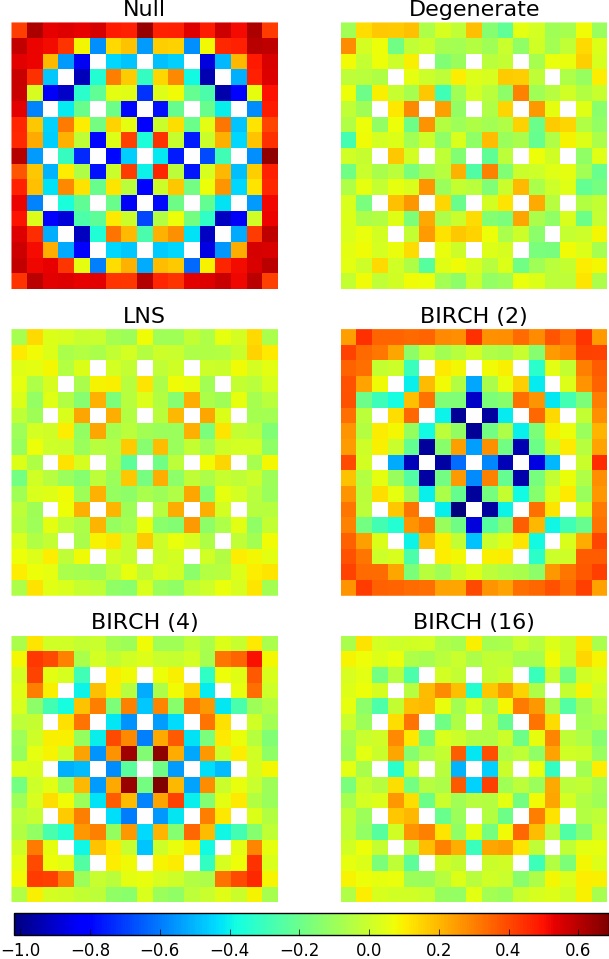
\includegraphics[width=0.87\linewidth]{figures/results/spatial/assm-31-20BPs/capt-err}
\vspace{2mm}
\caption[U-238 capture rate error spatial distributions]{U-238 capture percent relative errors for the 3.1\% enriched assembly with 20 \acp{BP} with null, degenerate, \ac{LNS} and \textit{i}\ac{MGXS} spatial homogenization.}
\label{fig:chap11-assm-3.1-20BPs-capt-err}
\end{figure}

\clearpage

\begin{figure}[h!]
\centering
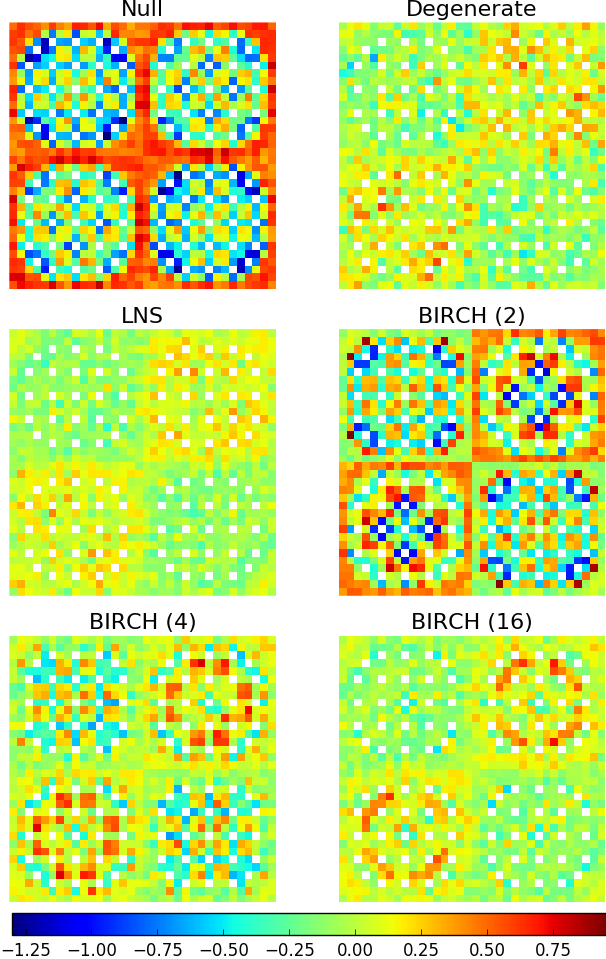
\includegraphics[width=0.87\linewidth]{figures/results/spatial/2x2/capt-err}
\vspace{2mm}
\caption[U-238 capture rate error spatial distributions]{U-238 capture percent relative errors for the 2$\times$2 colorset with null, degenerate, \ac{LNS} and \textit{i}\ac{MGXS} spatial homogenization.}
\label{fig:chap11-2x2-capt-err}
\end{figure}

\clearpage

\begin{figure}[h!]
\centering
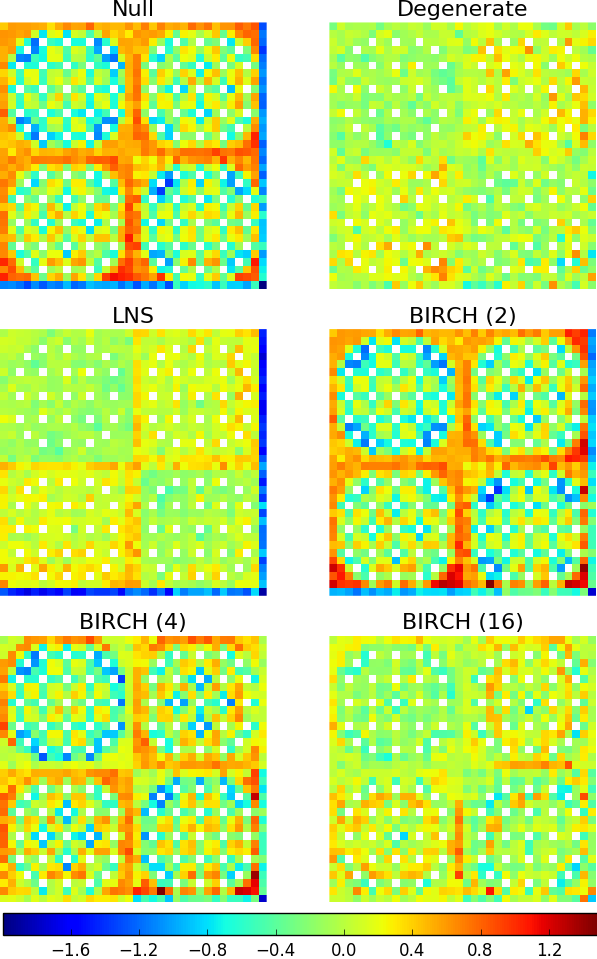
\includegraphics[width=0.87\linewidth]{figures/results/spatial/reflector/capt-err}
\vspace{2mm}
\caption[U-238 capture rate error spatial distributions]{U-238 capture percent relative errors for the 2$\times$2 colorset with a water reflector with null, degenerate, \ac{LNS} and \textit{i}\ac{MGXS} spatial homogenization.}
\label{fig:chap11-refl-capt-err}
\end{figure}

\clearpage

\begin{figure}[h!]
\centering
\begin{subfigure}{0.9\textwidth}
  \centering
  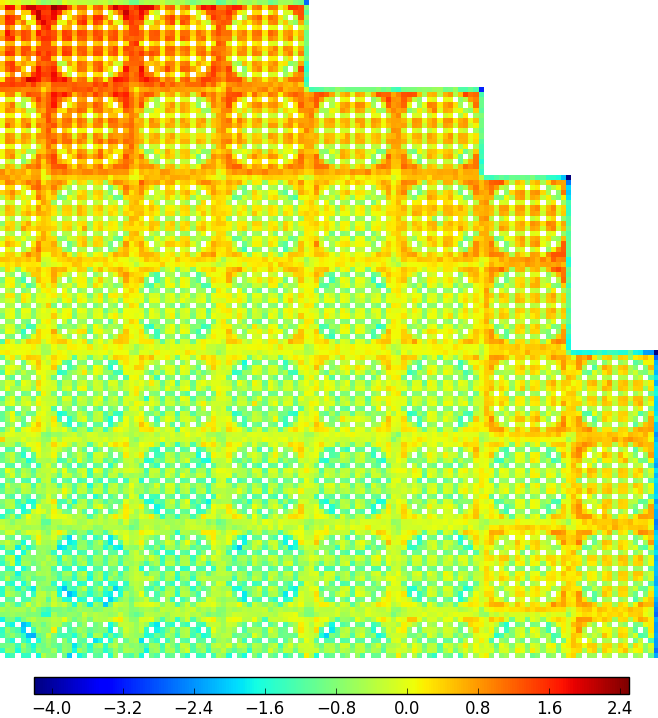
\includegraphics[width=0.65\linewidth]{figures/results/spatial/full-core/capt-err-null}
  \caption{}
  \label{fig:chap11-full-core-capt-err-null}
\end{subfigure}
\begin{subfigure}{0.9\textwidth}
  \centering
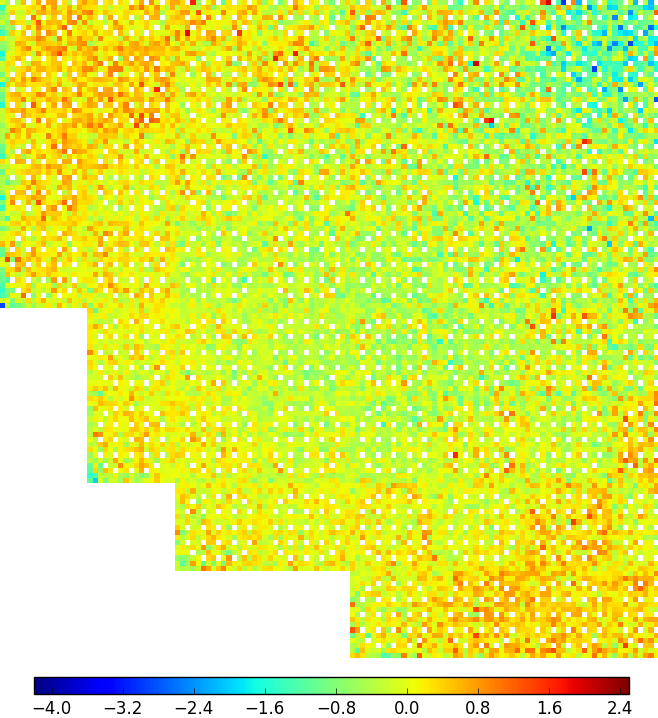
\includegraphics[width=0.65\linewidth]{figures/results/spatial/full-core/capt-err-degenerate}
  \caption{}
  \label{fig:chap11-full-core-capt-err-degenerate}
\end{subfigure}
\caption[U-238 capture rate error spatial distributions]{U-238 capture percent relative errors for the quarter core \ac{BEAVRS} model with null (a) and degenerate (b) spatial homogenization.}
\label{fig:chap11-full-core-capt-err-a}
\end{figure}

\clearpage

\begin{figure}[h!]
\centering
\begin{subfigure}{0.9\textwidth}
  \centering
  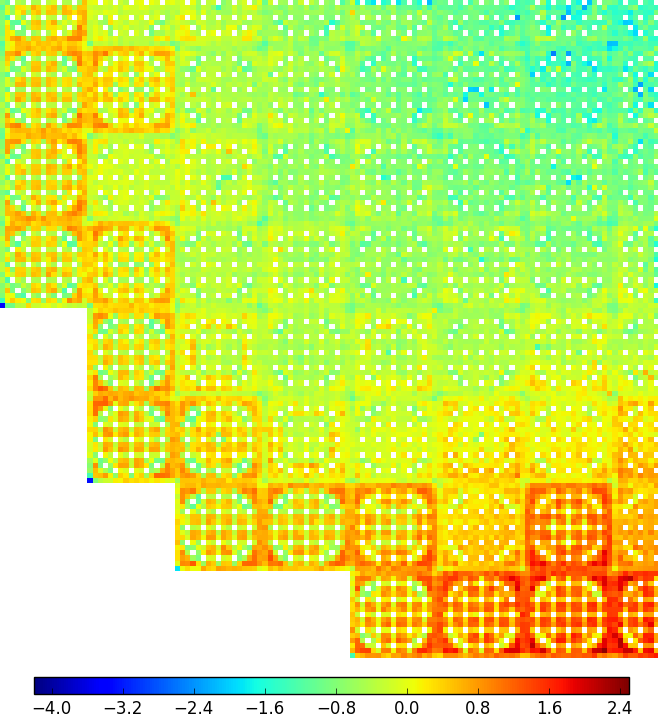
\includegraphics[width=0.65\linewidth]{figures/results/spatial/full-core/capt-err-birch-4}
  \caption{}
  \label{fig:chap11-full-core-capt-err-birch-4}
\end{subfigure}
\begin{subfigure}{0.9\textwidth}
  \centering
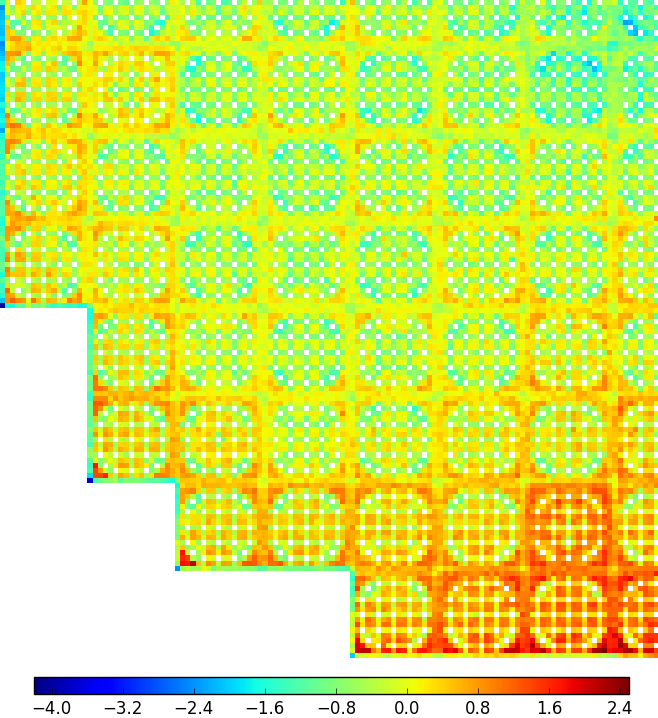
\includegraphics[width=0.65\linewidth]{figures/results/spatial/full-core/capt-err-birch-20}
  \caption{}
  \label{fig:chap11-full-core-capt-err-birch-16}
\end{subfigure}
\caption[U-238 capture rate error spatial distributions]{U-238 capture percent relative errors for the quarter core \ac{BEAVRS} model with \textit{i}\ac{MGXS} spatial homogenization with BIRCH clustering of 4 (a) and 20 (b) clusters.}
\label{fig:chap11-full-core-capt-err-b}
\end{figure}

\clearpage

%%%%%%%%%%%%%%%%%%%%%%%%%%%%%%%%%%%%%%%%%%%%%%%%%%%%%%%%%%%%%%%%%%
\subsubsection{Spatial Distributions of Capture-to-Fission Errors}
\label{subsec:chap11-imgxs-capt-to-fiss-errors}

\begin{figure}[h!]
\centering
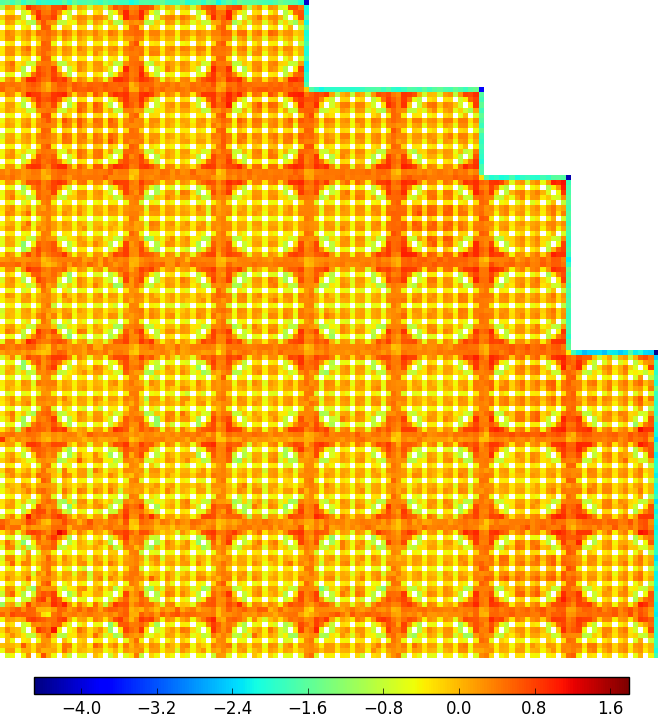
\includegraphics[width=0.65\linewidth]{figures/results/capt-to-fiss/spatial/full-core/capt-to-fiss-err-null}
\caption[Capture-to-fission rate error spatial distributions]{Percent relative errors on the U-238 capture to total fission rate ratio for the quarter core \ac{BEAVRS} model with null spatial homogenization.}
\label{fig:chap11-full-core-capt-to-fiss-err-null}
\end{figure}

\clearpage

\begin{figure}[h!]
\centering
\begin{subfigure}{0.9\textwidth}
  \centering
  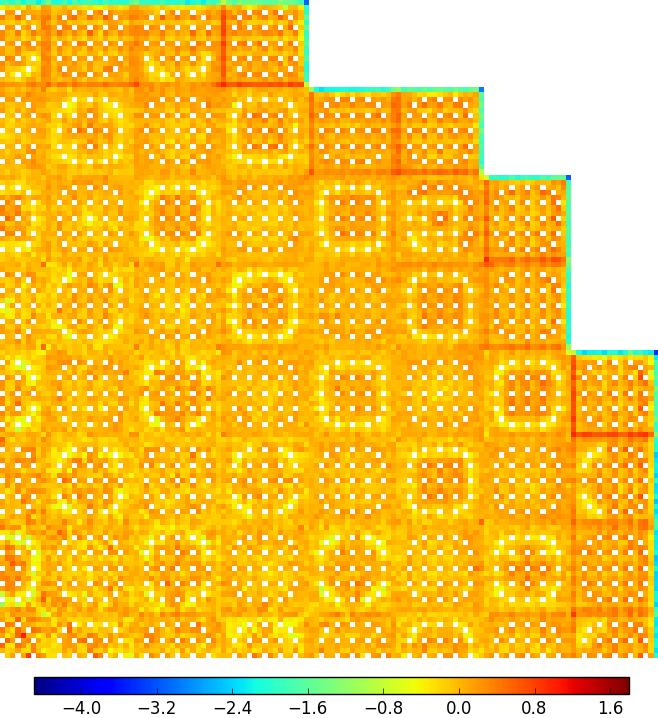
\includegraphics[width=0.65\linewidth]{figures/results/capt-to-fiss/spatial/full-core/capt-to-fiss-err-lns}
  \caption{}
  \label{fig:chap11-full-core-capt-to-fiss-err-lns}
\end{subfigure}
\begin{subfigure}{0.9\textwidth}
  \centering
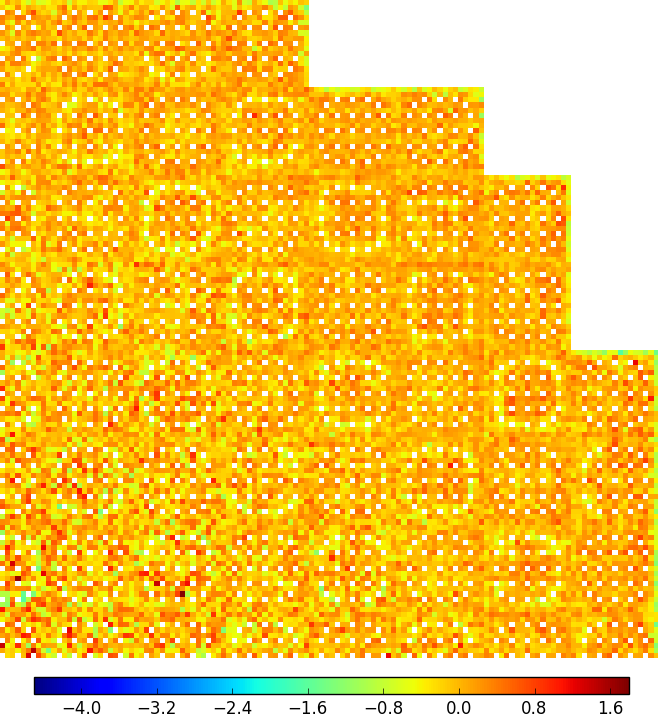
\includegraphics[width=0.65\linewidth]{figures/results/capt-to-fiss/spatial/full-core/capt-to-fiss-err-degenerate}
  \caption{}
  \label{fig:chap11-full-core-capt-to-fiss-err-degenerate}
\end{subfigure}
\caption[Capture-to-fission rate error spatial distributions]{Percent relative errors on the U-238 capture to total fission rate ratio for the quarter core \ac{BEAVRS} model with \ac{LNS} (a) and degenerate (b) spatial homogenization.}
\label{fig:chap11-full-core-capt-to-fiss-err-a}
\end{figure}

\clearpage

\begin{figure}[h!]
\centering
\begin{subfigure}{0.9\textwidth}
  \centering
  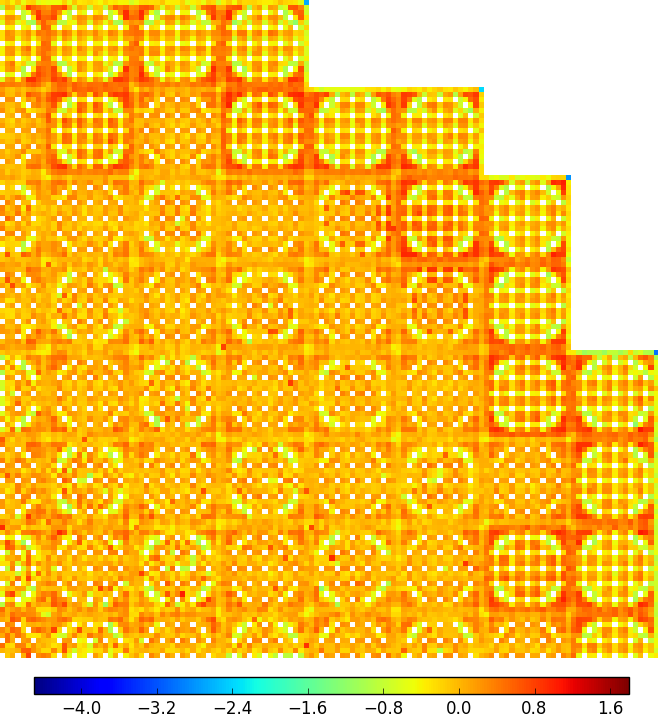
\includegraphics[width=0.65\linewidth]{figures/results/capt-to-fiss/spatial/full-core/capt-to-fiss-err-birch-4}
  \caption{}
  \label{fig:chap11-full-core-capt-to-fiss-err-birch-4}
\end{subfigure}
\begin{subfigure}{0.9\textwidth}
  \centering
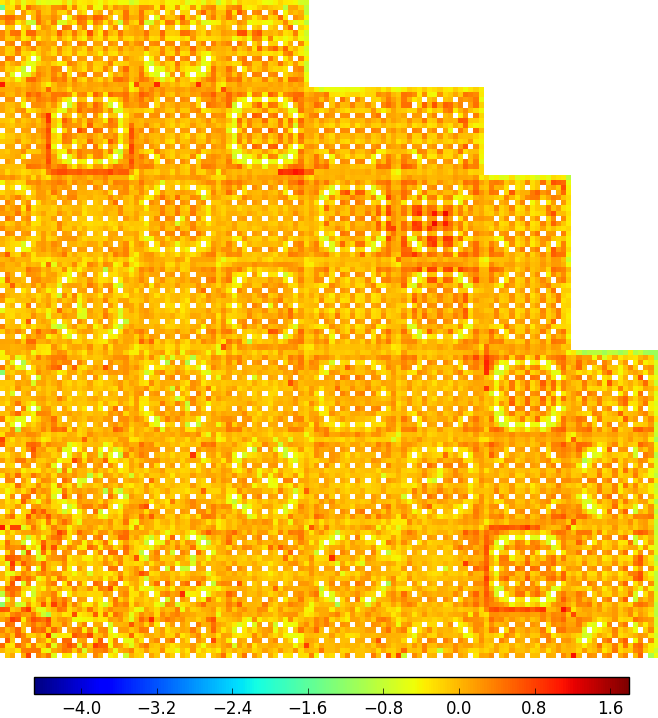
\includegraphics[width=0.65\linewidth]{figures/results/capt-to-fiss/spatial/full-core/capt-to-fiss-err-birch-20}
  \caption{}
  \label{fig:chap11-full-core-capt-to-fiss-err-birch-20}
\end{subfigure}
\caption[Capture-to-fission rate error spatial distributions]{Percent relative errors on the U-238 capture to total fission rate ratio for the quarter core \ac{BEAVRS} model with \textit{i}\ac{MGXS} spatial homogenization with BIRCH clustering of 4 (a) and 20 (b) clusters.}
\label{fig:chap11-full-core-capt-to-fiss-err-b}
\end{figure}

\clearpage

%%%%%%%%%%%%%%%%%%%%%%%%%%%%%%%%%%%%%%%%%%%
\subsubsection{A Comparison of OpenMOC Solutions}
\label{subsec:chap11-imgxs-capt-rates-compare}

This section directly compares the reaction rates from two different OpenMOC simulations with null and \textit{i}\ac{MGXS} homogenization to better understand the impact of \ac{MGXS} clustering on the spatial distribution of U-238 capture rate errors. In particular, the percent relative deviation $\Delta_{k}^{\mathrm{\textit{i}MGXS}}$ of the OpenMOC U-238 capture rate distributions between the null and \textit{i}\ac{MGXS} schemes is computed as follows:

\begin{equation}
\label{eqn:chap11-compare-openmoc}
\Delta_{k}^{\mathrm{\textit{i}MGXS}} \;\; [\%] \;\; = \;\; \frac{\left[\displaystyle\sum\limits_{g=1}^{G} \hat{\Sigma}^{238}_{\gamma,k,g}\phi_{k,g}\right]^{\mathrm{\textit{i}MGXS}} - \left[\displaystyle\sum\limits_{g=1}^{G} \hat{\Sigma}^{238}_{\gamma,k,g}\phi_{k,g}\right]^{\mathrm{Null}}}{\left[\displaystyle\sum\limits_{g=1}^{G} \hat{\Sigma}^{238}_{\gamma,k,g}\phi_{k,g}\right]^{\mathrm{Null}}} \times 100
\end{equation}

\noindent Unlike the U-238 capture rate error distributions, the relative deviations are not sensitive to the statistical uncertainties of the OpenMC reference solutions. As a result, it is easier to visualize the impact of clusters on the U-238 capture rate predictions. Figs.~\Crefrange{fig:chap11-assm-1.6-capt-rates-comp}{fig:chap11-refl-capt-rates-comp} present the percent relative deviations for the individual assembly and 2$\times$2 colorset benchmarks for BIRCH clustering of 2, 4, 8 and 16 clusters. Likewise, Figs.~\Crefrange{fig:chap11-full-core-capt-rates-kmeans-comp}{fig:chap11-full-core-capt-rates-birch-comp} illustrate the deviations for the quarter core \ac{BEAVRS} model with $k$-means, \ac{GMM} and BIRCH clustering of 4, 8, 16 and 20 clusters, respectively.

The figures illustrate the hierarchical nature of \ac{MGXS} clustering by discriminating fuel pins with different spatial self-shielding effects that occur in different regimes. For example, the first 2 clusters used for the individual assemblies distinguishes fuel pins which are adjacent (or nearly adjacent) to \acp{CRGT}, \acp{BP} or instrument tubes from those which are only surrounded by other fuel pins. The introduction of more clusters further refines these clusters to identify fuel pins with neighbors which have similar spatial self-shielding effects. For example, as the \textit{i}\ac{MGXS} scheme transitions between 8 -- 16 clusters for the 3.1\% enriched fuel assembly with 20 \acp{BP} (Fig.~\ref{fig:chap11-assm-31-20BPs-capt-rates-comp}), the fuel pins that are facially and diagonally adjacent to two \acp{CRGT} are separated into their own cluster. As a result, these eight fuel pins have the largest relative deviation from null homogenization since they experience the largest amount of moderation from the two \acp{CRGT}. Similarly, the first 2 -- 4 clusters in the colorset with a reflector (Fig.~\ref{fig:chap11-refl-capt-rates-comp}) discriminate pins along the assembly-assembly and assembly-reflector interfaces. As more clusters are introduced, they are increasingly customized to model the more local spatial self-shielding effects affecting the pins within the interior of each assembly due to the presence of \acp{CRGT} and \acp{BP}.

%As was noted in Sec.~\ref{subsec:chap11-imgxs-capt-rates-space-distrib}, the observations made here are specific to the configuration of the \textit{i}\ac{MGXS} data processing pipeline. The choice of features, dimensionality reduction technique(s) and clustering algorithm has a large impact on the clustering model and the resultant spatial distribution of U-238 capture rate errors, and should be further investigated in the future.

\begin{emphbox}
\textbf{The percent relative deviations between OpenMOC solutions with null and \textit{i}\ac{MGXS} homogenization makes it easy to discern the hierarchical nature of \ac{MGXS} clustering and its impact on U-238 capture rate predictions.}
\end{emphbox}

% than is possible with spatial distributions of errors with respect to a ``noisy'' Monte Carlo reference solution.

%-note a few outlier pins in the periodic colorset which break the symmetry

\begin{figure}[h!]
\centering
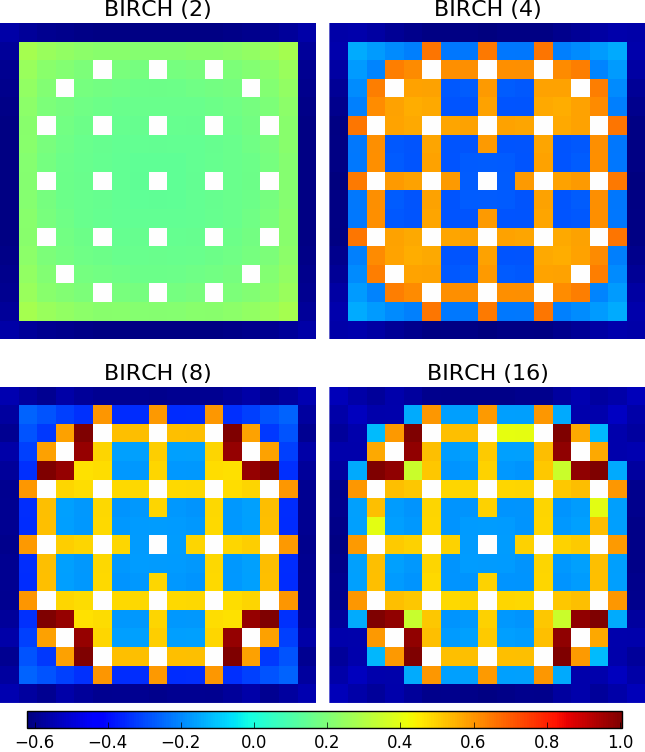
\includegraphics[width=0.9\linewidth]{figures/results/compare/assm-16/compare-capt}
\vspace{2mm}
\caption[U-238 capture rate \textit{i}MGXS-to-null relative deviations]{The percent relative deviation of U-238 capture rate spatial distributions for \textit{i}\ac{MGXS} and null homogenization for a 1.6\% enriched assembly.}
\label{fig:chap11-assm-1.6-capt-rates-comp}
\end{figure}

\clearpage

\begin{figure}[h!]
\centering
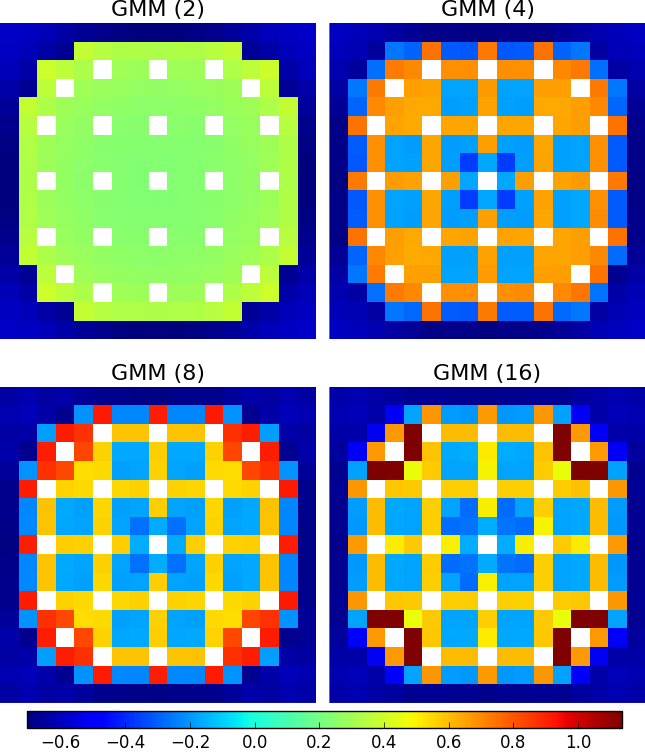
\includegraphics[width=0.9\linewidth]{figures/results/compare/assm-31/compare-capt}
\vspace{2mm}
\caption[U-238 capture rate \textit{i}MGXS-to-null relative deviations]{The percent relative deviation of U-238 capture rate spatial distributions for \textit{i}\ac{MGXS} and null homogenization for a 3.1\% enriched assembly.}
\label{fig:chap11-assm-3.1-capt-rates-comp}
\end{figure}

\clearpage

\begin{figure}[h!]
\centering
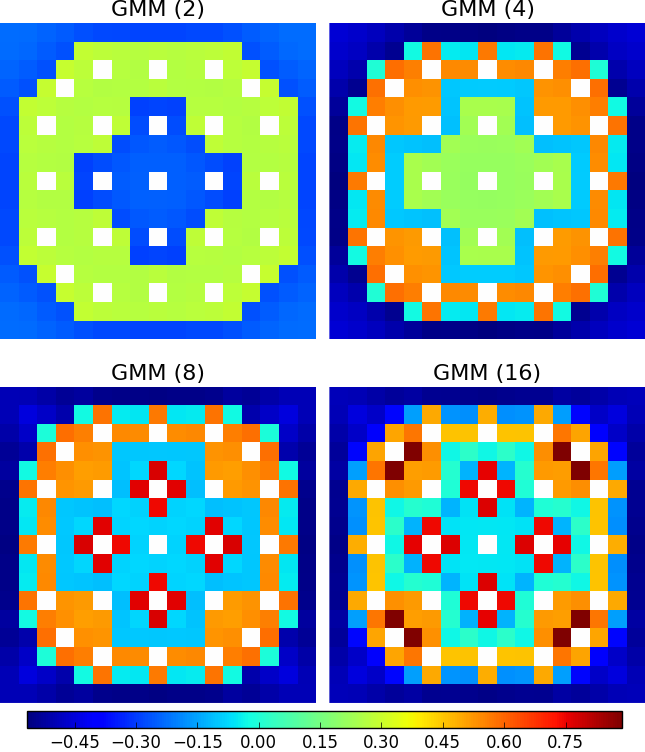
\includegraphics[width=0.9\linewidth]{figures/results/compare/assm-31-20BPs/compare-capt}
\vspace{2mm}
\caption[U-238 capture rate \textit{i}MGXS-to-null relative deviations]{The percent relative deviation of U-238 capture rate spatial distributions for \textit{i}\ac{MGXS} and null homogenization for a 3.1\% enriched assembly with 20 \acp{BP}.}
\label{fig:chap11-assm-31-20BPs-capt-rates-comp}
\end{figure}
	
\clearpage

\begin{figure}[h!]
\centering
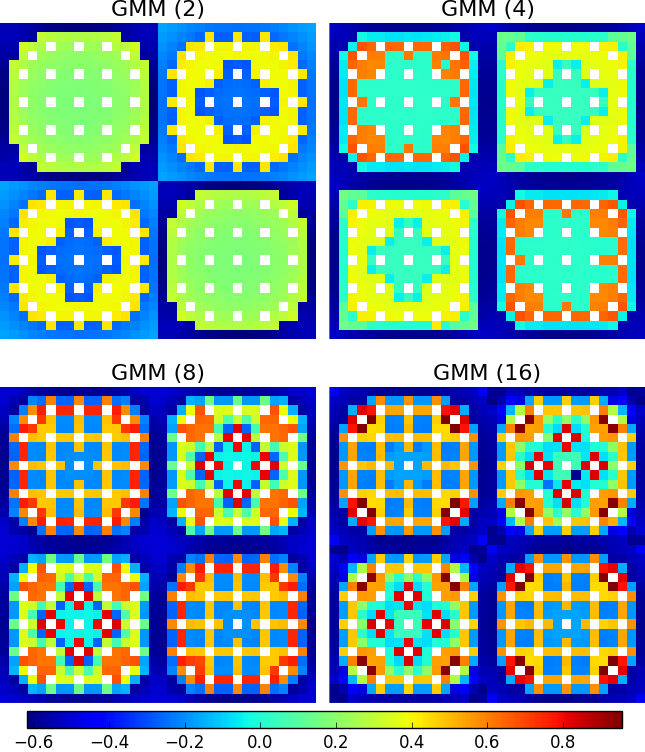
\includegraphics[width=0.9\linewidth]{figures/results/compare/2x2/compare-capt}
\vspace{2mm}
\caption[U-238 capture rate \textit{i}MGXS-to-null relative deviations]{The percent relative deviation of U-238 capture rate spatial distributions for \textit{i}\ac{MGXS} and null homogenization for a 2$\times$2 colorset.}
\label{fig:chap11-2x2-capt-rates-comp}
\end{figure}

\clearpage

\begin{figure}[h!]
\centering
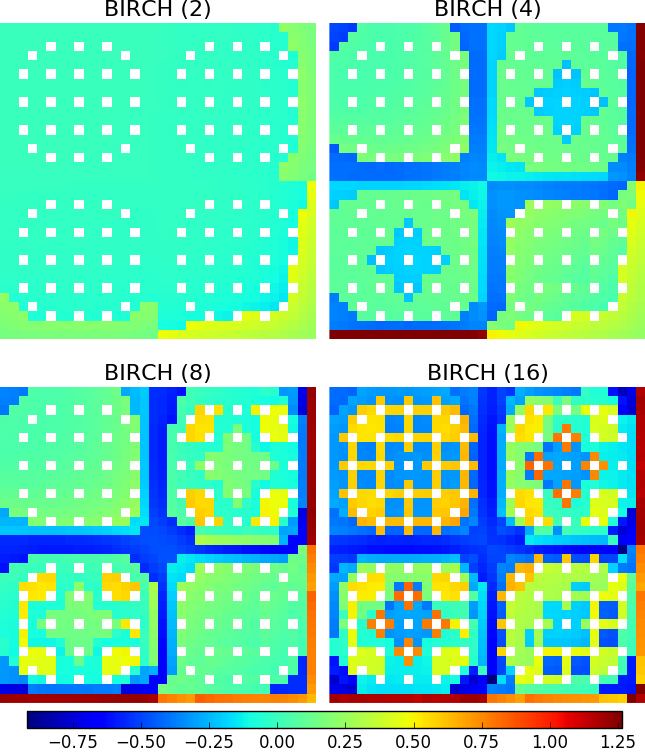
\includegraphics[width=0.9\linewidth]{figures/results/compare/reflector/compare-capt}
\vspace{2mm}
\caption[U-238 capture rate \textit{i}MGXS-to-null relative deviations]{The percent relative deviation of U-238 capture rate spatial distributions for \textit{i}\ac{MGXS} and null homogenization for a 2$\times$2 colorset with a water reflector.}
\label{fig:chap11-refl-capt-rates-comp}
\end{figure}

\clearpage

\begin{figure}[h!]
\centering
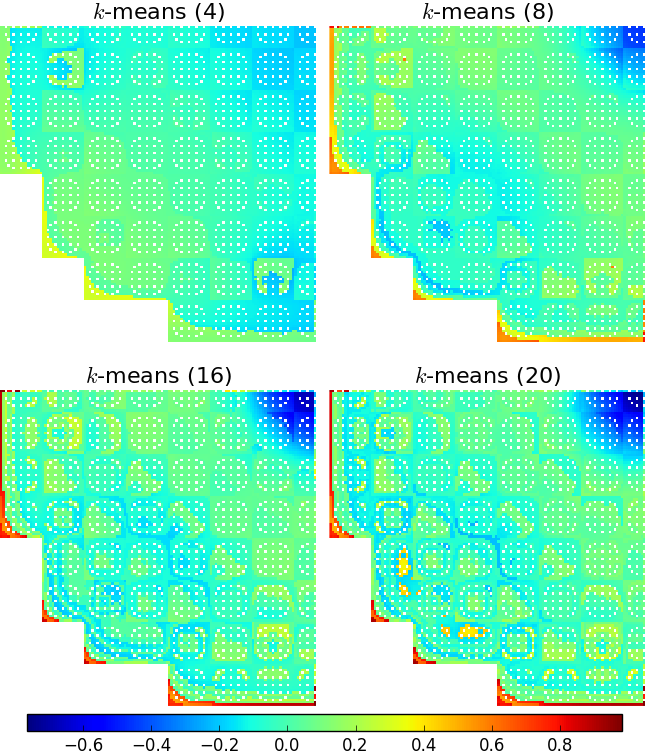
\includegraphics[width=0.9\linewidth]{figures/results/compare/full-core/compare-capt-kmeans}
\vspace{2mm}
\caption[U-238 capture rate \textit{i}MGXS-to-null relative deviations]{The percent relative deviation of U-238 capture rate spatial distributions for \textit{i}\ac{MGXS} (\textit{with $k$-means}) and null homogenization for the quarter core BEAVRS model.}
\label{fig:chap11-full-core-capt-rates-kmeans-comp}
\end{figure}

\clearpage

\begin{figure}[h!]
\centering
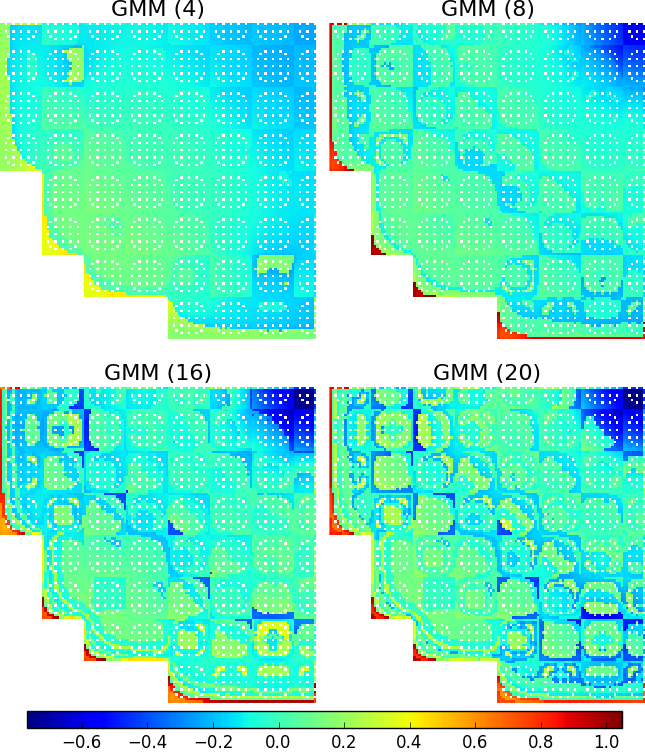
\includegraphics[width=0.9\linewidth]{figures/results/compare/full-core/compare-capt-gmm}
\vspace{2mm}
\caption[U-238 capture rate \textit{i}MGXS-to-null relative deviations]{The percent relative deviation of U-238 capture rate spatial distributions for \textit{i}\ac{MGXS} (\textit{with \ac{GMM}}) and null homogenization for the quarter core BEAVRS model.}
\label{fig:chap11-full-core-capt-rates-gmm-comp}
\end{figure}

\clearpage

\begin{figure}[h!]
\centering
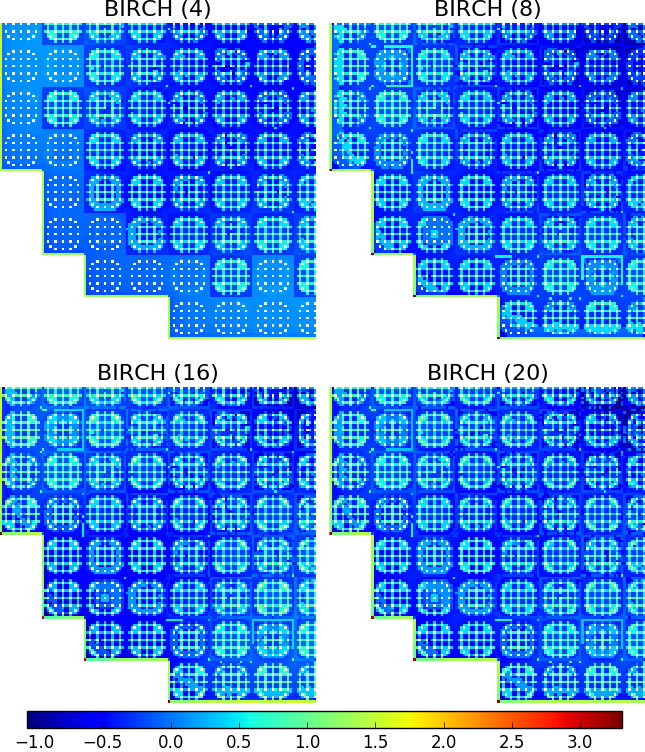
\includegraphics[width=0.9\linewidth]{figures/results/compare/full-core/compare-capt-birch}
\vspace{2mm}
\caption[U-238 capture rate \textit{i}MGXS-to-null relative deviations]{The percent relative deviation of U-238 capture rate spatial distributions for \textit{i}\ac{MGXS} (\textit{with BIRCH}) and null homogenization for the quarter core BEAVRS model.}
\label{fig:chap11-full-core-capt-rates-birch-comp}
\end{figure}

\clearpage


%%%%%%%%%%%%%%%%%%%%%%%%%%%%%%%%%%%%%%%%%%%%%%%%%%%%%%%%%%%%%%%%%%%%%%%%%%%%%%%
\section{Convergence of OpenMOC Solutions}
\label{sec:chap11-converge}

This section demonstrates how quickly multi-group solutions converge with number of \ac{MC} particle histories simulated to generate \ac{MGXS}. In particular, this section quantifies the number of histories needed to sufficiently converge \ac{MGXS} for stable OpenMOC solutions with the null, degenerate and \textit{i}\ac{MGXS} spatial homogenization schemes for each of the six benchmarks. In addition, the convergence of the OpenMOC solutions are compared to the statistical uncertainties of the corresponding reference OpenMC calculation. This comparison is used to quantify how much faster a solution for a specified accuracy can be achieved with OpenMOC with \ac{MGXS} generated by OpenMC.

This section uses the \ac{MC} tally data generated by the same OpenMC simulations which generated \ac{MGXS} for Sec.~\ref{subsec:chap11-imgxs-results}. However, the \ac{MGXS} in this section are computed from \ac{MC} tally data stored as OpenMC \textit{statepoint files} for 100 different active batches. For the assembly and colorset benchmarks, 80\% of the statepoints were recorded at a logarithmically-spaced interval for the first 1 -- 1,000 active batches (10$^{5}$ -- 10$^{8}$ histories), while the remaining 20\% were recorded at a logarithmically-spaced interval for the final 1,000 -- 9,800 active batches (10$^{8}$ -- 10$^{9}$ histories). The OpenMC statepoints for the earliest batches contained \ac{MC} tally data with the largest statistical uncertainties, while the tallies for the latter batches had smaller statistical uncertainties. The different statepoints enabled a thorough evaluation of the sensitivity of OpenMOC's solutions to the statistical uncertainties of the \ac{MGXS}.

\textbf{The clustering models were trained with the most highly converged \ac{MC} tally data stored for the final active batch} (\textit{i.e.}, the same data used to train the clustering models employed in Sec.~\ref{subsec:chap11-imgxs-results}). These clustering models were then re-applied for spatial homogenization of the lesser converged \ac{MC} tally data from earlier active batches. This methodology permitted a best case assessment of the OpenMOC accuracy one could hope to achieve if the ``best'' clustering model were accessible (\textit{i.e.}. the clustering model one would find from ``fully'' converged \ac{MC} tally data). It is important to note that this methodology is \textit{not} representative of how \textit{i}\ac{MGXS} would be deployed for \ac{MGXS} generation in a production setting. Nevertheless, it was a useful exercise to simply quantify the upper bound on the acceleration achievable if an optimal \textit{i}\ac{MGXS} configuration were invented which could infer reliable cluster assignments from highly unconverged \ac{MC} tally data.

%The objective for \textit{i}\ac{MGXS} is to infer accurate \ac{MGXS} cluster assignments for each fuel pin instance from ``noisy'' \ac{MC} tally data to accelerate the simulation scheme.

The convergence rate of the eigenvalues generated with null, degenerate and \textit{i}\ac{MGXS} homogenization is presented in Sec.~\ref{subsec:chap11-eigenvalue-converge}. Likewise, the convergence of the U-238 capture rate relative errors is examined in Sec.~\ref{subsec:chap11-capture-converge} for each scheme.

%%%%%%%%%%%%%%%%%%%%%%%%%%%%%%%%%%%
\subsection{Eigenvalue Convergence}
\label{subsec:chap11-eigenvalue-converge}

The OpenMOC eigenvalues were compared to the reference OpenMC eigenvalues from Tab.~\ref{table:chap7-ref-eigenvalues} for each of the 100 active batches. The eigenvalue bias $\Delta\rho$ was computed from Eqn.~\ref{eqn:chap5-delta-rho} in units of \ac{pcm}. The batch-by-batch bias is presented in Figs.~\Crefrange{fig:chap11-assm-1.6-eigenvalue-converge}{fig:chap11-refl-eigenvalue-converge} for the individual assembly and 2$\times$2 colorset benchmarks. In particular, the bias is presented for null, degenerate and \textit{i}\ac{MGXS} homogenization with BIRCH clustering of 2, 4 and 10 clusters for the assemblies and periodic colorset, and for 2, 4 and 16 clusters for the colorset with a water reflector. The biases are highlighted for 10$^{5}$ -- 10$^{9}$ active histories for the assemblies and 10$^{6}$ -- 10$^{9}$ histories for the colorsets, respectively\footnote{\label{converge}Several hundred thousand histories were required to sufficiently converge the \ac{MGXS} for the colorsets to compute stable solutions with OpenMOC.}.

The biases converge to nearly the same value for all of the benchmarks and spatial homogenization schemes, as expected based on the converged eigenvalue biases tabulated in Sec.~\ref{subsec:chap11-imgxs-eigenvalues}. This is consistent with the fact that globally-integrated reaction rates are preserved for all schemes irregardless of the number of clusters modeled. Of particular note is that the bias for the null and \textit{i}\ac{MGXS} schemes are quite consistent even with only 10$^{5}$ and 10$^{6}$ particle histories for the assembly and colorset benchmarks, respectively. The bias for the degenerate scheme deviates by up to 100 \ac{pcm}, but eventually converges to the null and \textit{i}\ac{MGXS} schemes with enough particle histories. The bias fluctuates on the order of 500 \ac{pcm} with fewer than 10$^{7}$ particle histories, but converges with 10$^{8}$ histories for all of the benchmarks and schemes.

A number of different factors may cause the eigenvalue to fluctuate and deviate between schemes for few particle histories. First, the statistical uncertainties of the \ac{MGXS} must be minimized in order to converge the OpenMOC eigenvalues. In addition, it should be recalled from Sec.~\ref{sec:chap3-mgxs-gen} that the \ac{MGXS} are generated from OpenMC using a mixture of track-length and analog tally estimators. In particular, the total, fission and capture \ac{MGXS} are computed with track-length estimators, while the scattering matrices and fission spectra are computed from analog estimators since they depend on the neutron's outgoing energy at each interaction. Although both track-length and analog estimators will converge to the same expected value, analog estimators will converge more slowly. As a result, neutron balance will not be preserved for \ac{MGXS} computed from a mixture of track-length and analog estimators without a sufficient number of simulated histories. This issue was the a key motivating factor for Nelson's Nuclear Data PreProcessor (NDPP)~\cite{nelson2014improved} to enable track-length estimators for multi-group scattering matrices and fission spectra. Methods  such as NDPP may be a fruitful area of future research to enable faster converging eigenvalues from \ac{MGXS} generated with \ac{MC}.

\begin{emphbox}
\textbf{The null, degenerate and \textit{i}\ac{MGXS} schemes converge to the same eigenvalue bias with 10$^{8}$ particle histories for the assembly and colorset benchmarks.}
\end{emphbox}

%-why do the plots start at 10^5 for the assemblies, and 10^6 for the colorsets???
%  -because 100,000 particles led to NaNs for the reflector and colorset benchmarks

\begin{figure}[h!]
\centering
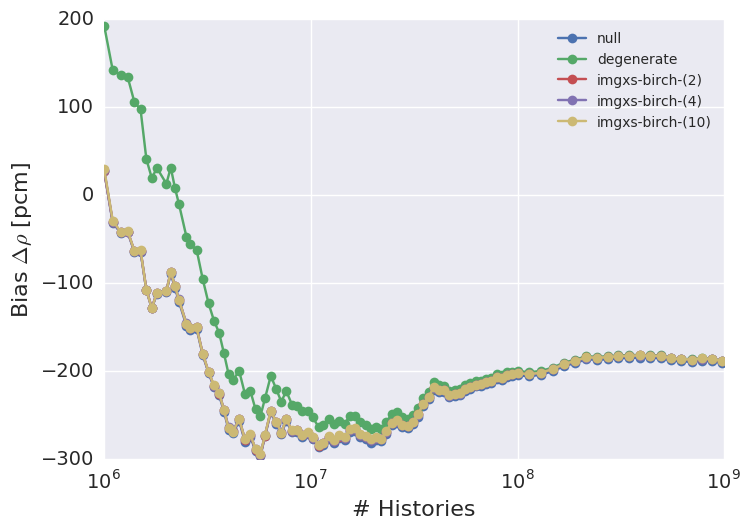
\includegraphics[width=0.88\linewidth]{figures/results/convergence/assm-16/keff-bias-evo}
\vspace{2mm}
\caption[Eigenvalue bias convergence with MC histories]{Convergence of the eigenvalue bias for the 1.6\% enriched assembly.}
\label{fig:chap11-assm-1.6-eigenvalue-converge}
\end{figure}

\begin{figure}[h!]
\centering
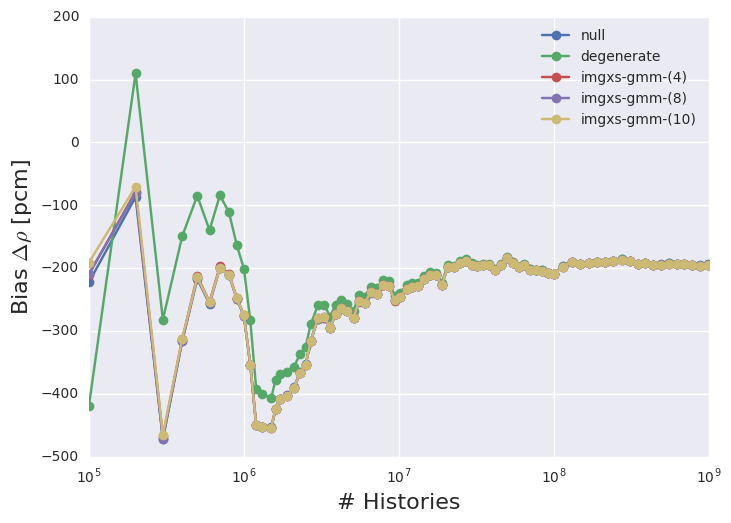
\includegraphics[width=0.88\linewidth]{figures/results/convergence/assm-31/keff-bias-evo}
\vspace{2mm}
\caption[Eigenvalue bias convergence with MC histories]{Convergence of the eigenvalue bias for the 3.1\% enriched assembly.}
\label{fig:chap11-assm-3.1-eigenvalue-converge}
\end{figure}

\begin{figure}[h!]
\centering
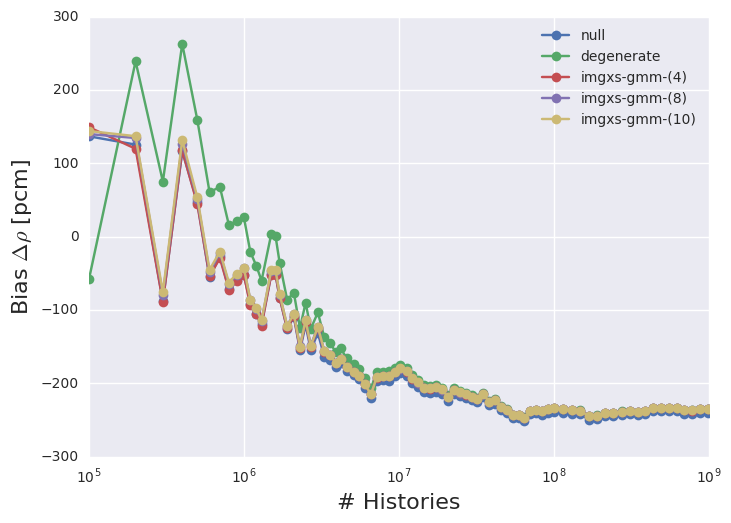
\includegraphics[width=0.88\linewidth]{figures/results/convergence/assm-31-20BPs/keff-bias-evo}
\vspace{2mm}
\caption[Eigenvalue bias convergence with MC histories]{Convergence of the eigenvalue bias for the 3.1\% enriched assembly with 20 \acp{BP}.}
\label{fig:chap11-assm-3.1-20BPs-eigenvalue-converge}
\end{figure}

\begin{figure}[h!]
\centering
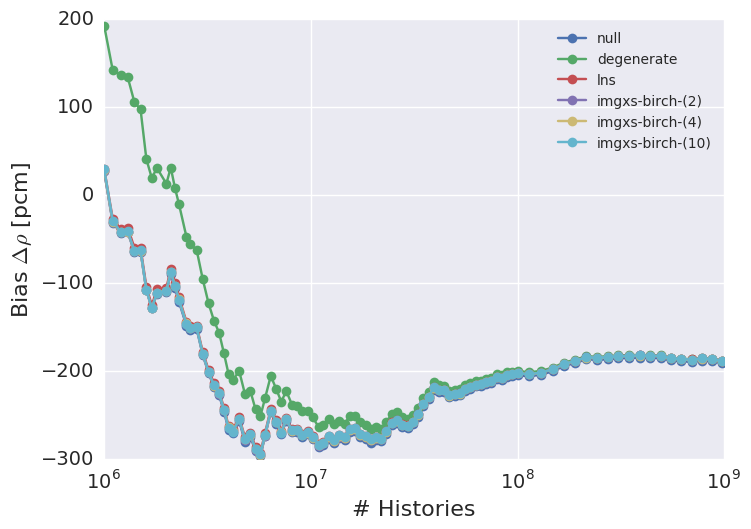
\includegraphics[width=0.88\linewidth]{figures/results/convergence/2x2/keff-bias-evo}
\vspace{2mm}
\caption[Eigenvalue bias convergence with MC histories]{Convergence of the eigenvalue bias for the periodic colorset.}
\label{fig:chap11-2x2-eigenvalue-converge}
\end{figure}

\begin{figure}[h!]
\centering
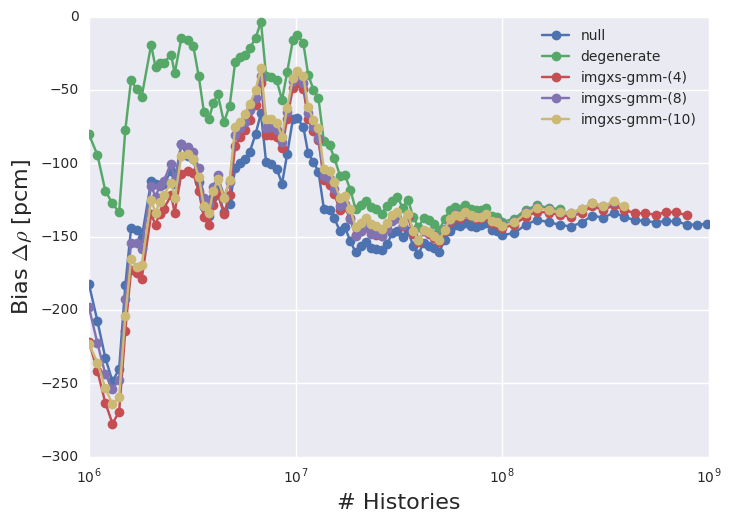
\includegraphics[width=0.88\linewidth]{figures/results/convergence/reflector/keff-bias-evo}
\vspace{2mm}
\caption[Eigenvalue bias convergence with MC histories]{Convergence of the eigenvalue bias for the colorset with a water reflector.}
\label{fig:chap11-refl-eigenvalue-converge}
\end{figure}

\clearpage

%%%%%%%%%%%%%%%%%%%%%%%%%%%%%%%%%%%%%%%%%%%
\subsection{U-238 Capture Rate Convergence}
\label{subsec:chap11-capture-converge}

The OpenMOC energy-integrated pin-wise U-238 capture rates were compared to the reference OpenMC capture rates to compute the percent relative errors for each pin's capture rates for each of the 100 active batches. The batch-by-batch maximum and mean relative errors are presented in Figs.~\Crefrange{fig:chap11-assm-1.6-capture-converge}{fig:chap11-refl-capture-converge} for the individual assembly and 2$\times$2 colorset benchmarks. In particular, the errors are presented for null, degenerate and \textit{i}\ac{MGXS} homogenization with BIRCH clustering of 2, 4 and 10 clusters for the assemblies and periodic colorset, and for 2, 4 and 16 clusters for the colorset with a water reflector. In addition, the maximum and mean statistical uncertainty (1-sigma) of the OpenMC estimate for the pin-wise U-238 capture rates is also highlighted in each figure\footnote{Although the OpenMOC relative error and OpenMC statistical uncertainty are not equivalent, it is useful to compare their convergence rates as a proxy for the relative runtimes of directly computing a reference solution with OpenMC, versus using OpenMC to generate sufficiently converged \ac{MGXS} for OpenMOC.}. The OpenMOC errors and OpenMC uncertainties are highlighted for 10$^{5}$ -- 10$^{9}$ active histories for the assemblies and 10$^{6}$ -- 10$^{9}$ histories for the colorsets, respectively\textsuperscript{\ref{converge}}.

% . If the OpenMC uncertainty were to converge faster, then it would make more sense to compute eigenvalues and reaction rate distributions directly from OpenMC simulations, instead of using it to generate \ac{MGXS} for OpenMOC. Alternatively, if the OpenMOC solutions  converge more quickly than OpenMC -- which is assumed as the basis for this thesis -- then }.

A couple of key conclusions can be drawn from these results. First, the OpenMC statistical uncertainties converge at a rate similar to the OpenMOC errors for degenerate homogenization. The maximum OpenMC uncertainty is always less than the maximum degenerate error. However, the mean uncertainty is greater than the mean degenerate error for fewer than approximately 500,000,000 histories. With a sufficient number of histories, the uncertainties fall below the errors. The OpenMC uncertainties approach zero while the OpenMOC errors approach a non-zero bias dependent on the approximation error separating the OpenMOC and reference OpenMC solutions. The final converged errors illustrate the same behavior as discussed in Sec.~\ref{subsec:chap11-imgxs-capt-rates}. In particular, the converged \textit{i}\ac{MGXS} errors increasingly approach the degenerate errors as more clusters are introduced. While the degenerate scheme always outperforms \textit{i}\ac{MGXS}, the improvement is relatively marginal compared to the improvement that \textit{i}\ac{MGXS} achieves with respect to the null scheme.

Both the maximum and mean errors for the null homogenization scheme are converged with only 10$^{5}$ and 10$^{6}$ histories for the assembly and colorset benchmarks, respectively. In contrast, the errors for the degenerate scheme are not fully converged even with 10$^{9}$ histories. This indicates that at least some fraction of the OpenMOC relative errors with the degenerate scheme is due to the lingering statistical uncertainties of the \ac{MGXS}. The degenerate error would only converge if more particle histories were simulated to compute the \ac{MGXS}. The convergence of the \textit{i}\ac{MGXS} scheme lies between that of the null and degenerate schemes, and requires more particle histories to converge as more clusters are identified. The convergence behavior is increasingly erratic with more histories, as is illustrated by the maximum error of the \textit{i}\ac{MGXS} scheme with 16 clusters for the colorset with water reflector in Fig.~\ref{fig:chap11-refl-capture-converge-max}.
 
%First, the mean error is more smoothly converging than the maximum error for all benchmarks. 

The figures illustrate the potential for \textit{i}\ac{MGXS} to achieve nearly the same accuracy as the degenerate scheme with a factor of 10 or fewer particle histories. Furthermore, the results indicate that OpenMOC's errors converge at least 10$\times$ faster than OpenMC's statistical uncertainties converge to the same value.

\begin{emphbox}
\textbf{The OpenMOC U-238 capture rate errors with null homogenization converge with fewer than 10$^{6}$ histories, while the errors with degenerate homogenization are not converged even with 10$^{9}$ histories. The convergence rate of the errors decreases with the number of clusters used in \textit{i}\ac{MGXS} spatial homogenization. The \textit{i}\ac{MGXS} scheme requires 10$\times$ fewer particle histories to converge than both the degenerate scheme and the OpenMC reference solution.}
\end{emphbox}

%    -would be interesting to look at alternatives to track density-weighting
%    -how about taking the median MGXS from each cluster?
%      -would be less sensitive to outliers and potentially more ``robust''
%      -but wouldn't preserve global reactivity
%    -recall argument about LNS - uneven number of fuel pin instances assigned to each cluster
%      -clusters with the fewest pins will be most constraining on convergence

\begin{figure}[h!]
\centering
\begin{subfigure}{\textwidth}
  \centering
  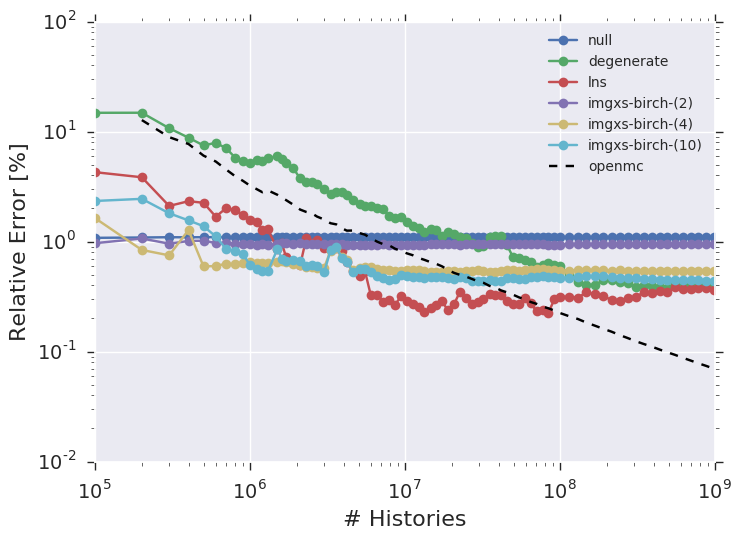
\includegraphics[width=0.9\linewidth]{figures/results/convergence/assm-16/max-capt-err-evo}
  \caption{}
  \label{fig:chap11-assm-1.6-capture-converge-max}
\end{subfigure}
\begin{subfigure}{\textwidth}
  \centering
  \includegraphics[width=0.9\linewidth]{figures/results/convergence/assm-16/mean-capt-err-evo}
  \caption{}
  \label{fig:chap11-assm-1.6-capture-converge-mean}
\end{subfigure}
\vspace{2mm}
\caption[U-238 capture rate error convergence with MC histories]{Convergence of the max (a) and mean (b) absolute U-238 capture rate percent relative errors for the 1.6\% enriched assembly.}
\label{fig:chap11-assm-1.6-capture-converge}
\end{figure}

\begin{figure}[h!]
\centering
\begin{subfigure}{\textwidth}
  \centering
  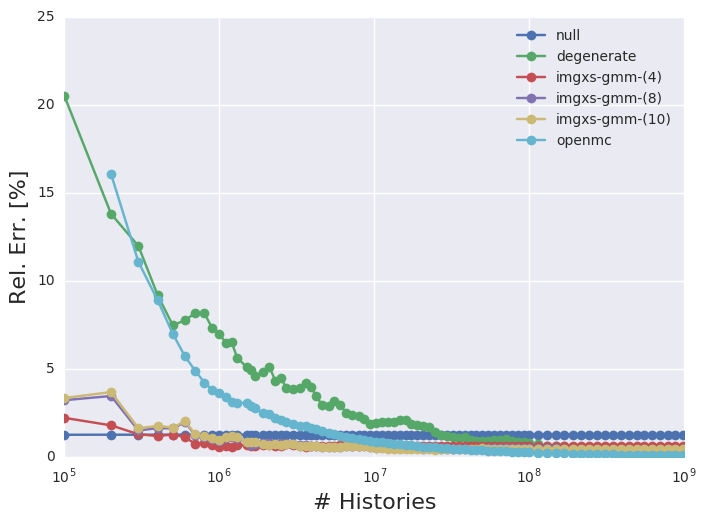
\includegraphics[width=0.9\linewidth]{figures/results/convergence/assm-31/max-capt-err-evo}
  \caption{}
  \label{fig:chap11-assm-3.1-capture-converge-max}
\end{subfigure}
\begin{subfigure}{\textwidth}
  \centering
  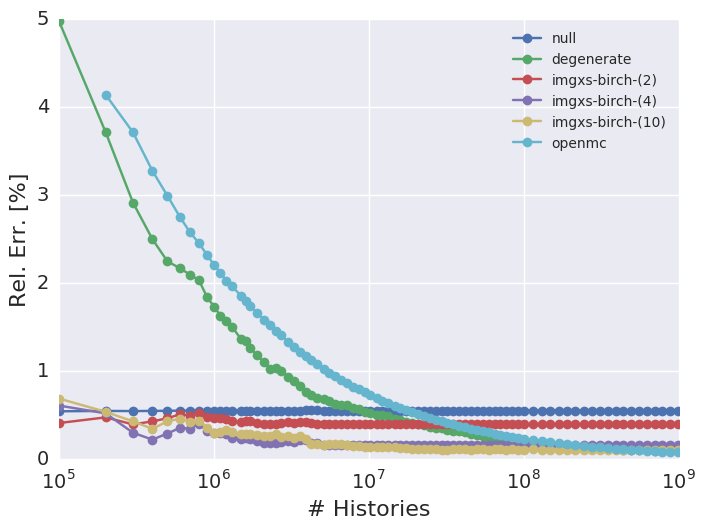
\includegraphics[width=0.9\linewidth]{figures/results/convergence/assm-31/mean-capt-err-evo}
  \caption{}
  \label{fig:chap11-assm-3.1-capture-converge-mean}
\end{subfigure}
\vspace{2mm}
\caption[U-238 capture rate error convergence with MC histories]{Convergence of the max (a) and mean (b) absolute U-238 capture rate percent relative errors for the 3.1\% enriched assembly.}
\label{fig:chap11-assm-3.1-capture-converge}
\end{figure}

\begin{figure}[h!]
\centering
\begin{subfigure}{\textwidth}
  \centering
  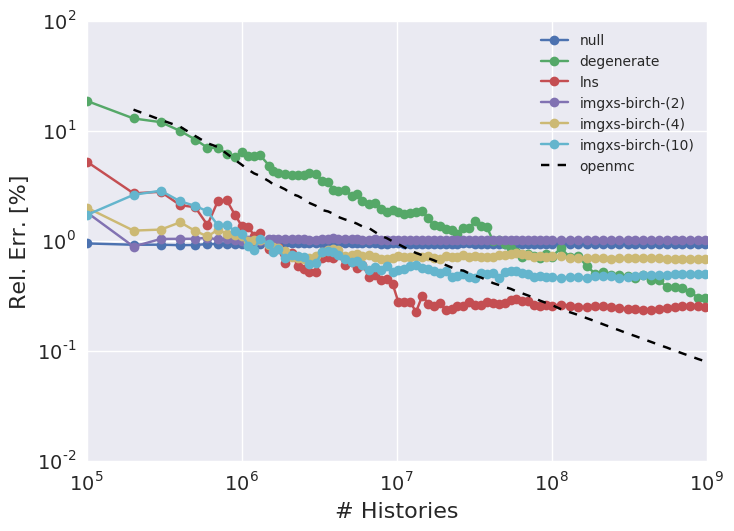
\includegraphics[width=0.9\linewidth]{figures/results/convergence/assm-31-20BPs/max-capt-err-evo}
  \caption{}
  \label{fig:chap11-assm-3.1-20BPs-capture-converge-max}
\end{subfigure}
\begin{subfigure}{\textwidth}
  \centering
  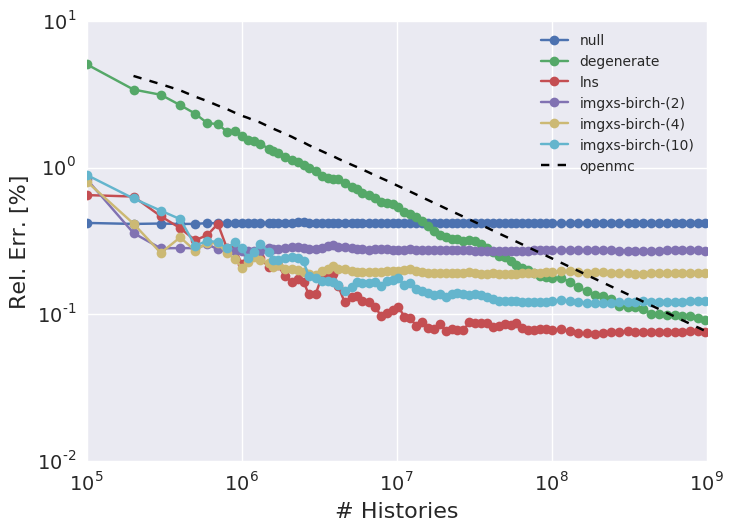
\includegraphics[width=0.9\linewidth]{figures/results/convergence/assm-31-20BPs/mean-capt-err-evo}
  \caption{}
  \label{fig:chap11-assm-3.1-20BPs-capture-converge-mean}
\end{subfigure}
\vspace{2mm}
\caption[U-238 capture rate error convergence with MC histories]{Convergence of the max (a) and mean (b) absolute U-238 capture rate percent relative errors for the 3.1\% enriched assembly with 20 \acp{BP}.}
\label{fig:chap11-assm-3.1-20BPs-capture-converge}
\end{figure}

\begin{figure}[h!]
\centering
\begin{subfigure}{\textwidth}
  \centering
  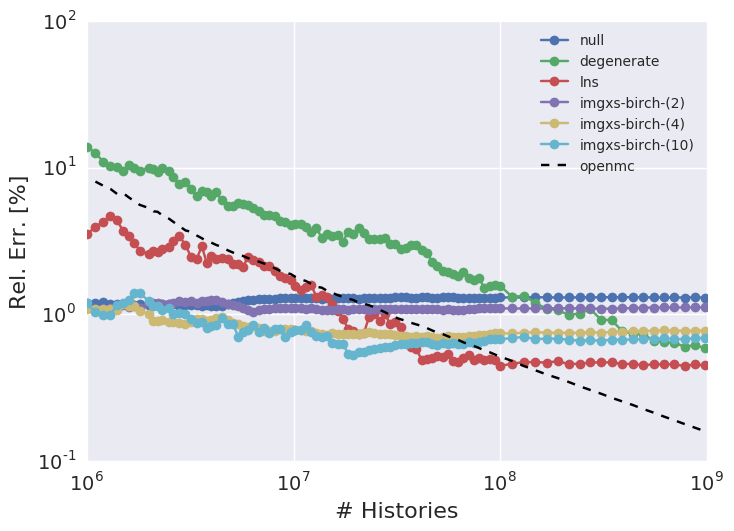
\includegraphics[width=0.9\linewidth]{figures/results/convergence/2x2/max-capt-err-evo}
  \caption{}
  \label{fig:chap11-2x2-capture-converge-max}
\end{subfigure}
\begin{subfigure}{\textwidth}
  \centering
  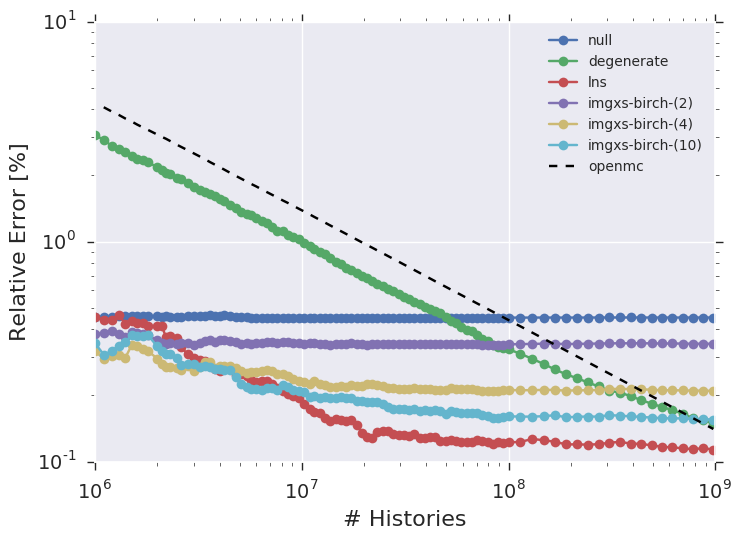
\includegraphics[width=0.9\linewidth]{figures/results/convergence/2x2/mean-capt-err-evo}
  \caption{}
  \label{fig:chap11-2x2-capture-converge-mean}
\end{subfigure}
\vspace{2mm}
\caption[U-238 capture rate error convergence with MC histories]{Convergence of the max (a) and mean (b) absolute U-238 capture rate percent relative errors for the periodic colorset.}
\label{fig:chap11-2x2-capture-converge}
\end{figure}

\begin{figure}[h!]
\centering
\begin{subfigure}{\textwidth}
  \centering
  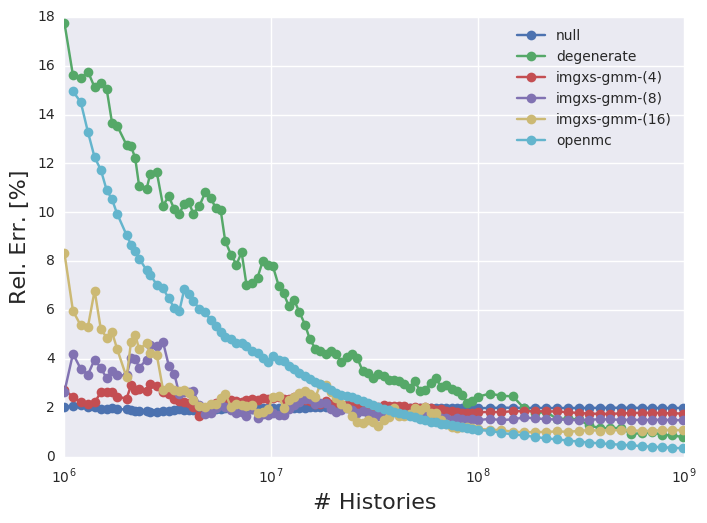
\includegraphics[width=0.9\linewidth]{figures/results/convergence/reflector/max-capt-err-evo}
  \caption{}
  \label{fig:chap11-refl-capture-converge-max}
\end{subfigure}
\begin{subfigure}{\textwidth}
  \centering
  \includegraphics[width=0.9\linewidth]{figures/results/convergence/reflector/mean-capt-err-evo}
  \caption{}
  \label{fig:chap11-refl-capture-converge-mean}
\end{subfigure}
\vspace{2mm}
\caption[U-238 capture rate error convergence with MC histories]{Convergence of the max (a) and mean (b) absolute U-238 capture rate percent relative errors for the colorset with a water reflector.}
\label{fig:chap11-refl-capture-converge}
\end{figure}

\clearpage


%%%%%%%%%%%%%%%%%%%%%%%%%%%%%%%%%%%%%%%%%%%%%%%%%%%%%%%%%%%%%%%%%%%%%%%%%%%%%%%
\section{Evaluation of Model Selection Techniques}
\label{sec:chap11-model-select}

This section analyzes the model selection criteria introduced in Sec.~\ref{sec:chap10-model-select}. The various criteria are computed for the clustering models trained in Sec.~\ref{subsec:chap11-imgxs-capt-rates-num-clusters}. The model selection criteria are designed to quantitatively compare clustering models, and in particular, to help choose the optimal number of clusters. In a truly unsupervised (\textit{i.e.}, production) setting, the OpenMOC eigenvalue bias and reaction rate errors with respect to a reference OpenMC solution would not be available to help choose the optimal number of clusters. Instead, the ``best'' clustering model would be chosen strictly from the model selection criteria.

Each criterion was computed for the clustering models built for the 1.6\% enriched fuel assembly and 2$\times$2 colorset with water reflector. The Davies-Bouldin, Dunn and Calinski-Harabaz indices are presented in Secs.~\Crefrange{subsec:chap11-db-index}{subsec:chap11-ch-index}, respectively. The silhouette coefficients are presented in Sec.~\ref{subsec:chap11-silhouette-coeff}. Finally, Sec.~\ref{subsec:chap11-bic} highlights the Bayesian Information Criterion (BIC) for the \ac{GMM} clustering algorithm. Cross-validation (Sec.~\ref{subsec:chap10-cross-validate}) was not employed to compute the heuristics, but could be used in the future to compute more robust estimates for each criterion.	

%-could compare cluster labels to those from LNS (use LNS as the ``ground truth'')

%%%%%%%%%%%%%%%%%%%%%%%%%%%%%%%%%
\subsection{Davies-Bouldin Index}
\label{subsec:chap11-db-index}

The Davies-Bouldin (DB) index is the ratio of within-cluster scatter to between-cluster separation (Sec.~\ref{subsec:chap10-db-index}), and is presented in Fig.~\ref{fig:chap11-db-indices}. In theory, the ``best'' clustering model should minimize the DB index. The figures illustrate that the smallest DB indices correspond to the clustering models with two clusters\footnote{The Davies-Bouldin index is undefined for a single cluster.}. As more clusters are added to each model, the within-cluster scatter should decrease, while the between-cluster separation should increase. The increasing DB indices indicate that the within-cluster scatter decreases more slowly than the between-cluster separation increases for both benchmarks. It is unclear why the DB index behaves in this way. Furthermore, it is not clear that the DB index would be a useful metric for determining the optimal number of clusters since it would only choose two clusters for both benchmarks.

\begin{figure}[h!]
\centering
\begin{subfigure}{\textwidth}
  \centering
  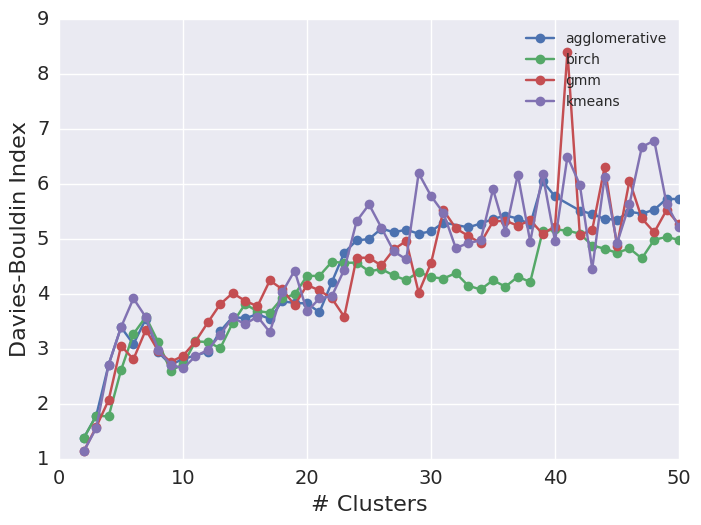
\includegraphics[width=0.9\linewidth]{figures/results/model-select/assm-16/db-combined-U238-capture-1}
  \caption{}
  \label{fig:chap11-assm-16-db-index}
\end{subfigure}
\begin{subfigure}{\textwidth}
  \centering
  \includegraphics[width=0.9\linewidth]{figures/results/model-select/reflector/db-combined-U238-nu-fission-1}
  \caption{}
\label{fig:chap11-refl-db-index}
\end{subfigure}
\caption[Davies-Bouldin index variation with the number of clusters]{Davies-Bouldin indices for the 1.6\% enriched assembly (a) and 2$\times$2 colorset with a water reflector (b) for each of the four clustering algorithms.}
\label{fig:chap11-db-indices}
\end{figure}

\clearpage

%%%%%%%%%%%%%%%%%%%%%%%
\subsection{Dunn Index}
\label{subsec:chap11-dunn-index}

The Dunn index is the ratio of the minimum inter-cluster distance to the maximum intra-cluster distance (Sec.~\ref{subsec:chap10-dunn-index}), and is presented in Fig.~\ref{fig:chap11-dunn-indices}. The Dunn indices are only highlighted for 3 -- 50 clusters since the index was over five orders of magnitude larger for only two clusters, which would not be useful to plot alongside the indices for more clusters\footnote{The Dunn index is undefined for a single cluster.}. In theory, the ``best'' clustering model should maximize the Dunn index. The clustering models with only two clusters maximize the Dunn index. As more clusters are added to each model, both the minimum inter-cluster and maximum intra-cluster distances should decrease. The decreasing Dunn indices indicate that the minimum inter-cluster distance decreases more slowly than the maximum intra-cluster distance for both benchmarks. It is unclear why the Dunn index behaves in this way. Furthermore, it is not clear that the Dunn index would be a useful metric for determining the optimal number of clusters since it would only choose two clusters for both benchmarks. Nevertheless, it should be recalled that the Dunn index is designed to characterize the most poorly defined cluster(s) in the model. The Dunn index varies in a step-like fashion in the figures, indicating that the most poorly defined cluster(s) are not typically refined with each successive cluster added to the models.

\begin{figure}[h!]
\centering
\begin{subfigure}{\textwidth}
  \centering
\includegraphics[width=0.9\linewidth]{figures/results/model-select/assm-16/dunn-combined-U238-capture-1}
\vspace{2mm}
  \caption{}
  \label{fig:chap11-assm-16-dunn-index}
\end{subfigure}
\begin{subfigure}{\textwidth}
  \centering
\includegraphics[width=0.9\linewidth]{figures/results/model-select/reflector/dunn-combined-U238-nu-fission-1}
  \caption{}
\label{fig:chap11-refl-dunn-index}
\end{subfigure}
\caption[Dunn index variation with the number of clusters]{Dunn indices for the 1.6\% enriched assembly (a) and 2$\times$2 colorset with a water reflector (b) for each of the four clustering algorithms.}
\label{fig:chap11-dunn-indices}
\end{figure}

\clearpage

%%%%%%%%%%%%%%%%%%%%%%%%%%%%%%%%%%%
\subsection{Calinski-Harabaz Index}
\label{subsec:chap11-ch-index}

The Calinski-Harabaz (CH) index is the ratio of between-cluster and within-cluster dispersion (Sec.~\ref{subsec:chap10-calinski-harabaz}) and is presented in Fig.~\ref{fig:chap11-ch-indices}. In theory, the ``best'' clustering model should maximize the CH index. The figures illustrate that the largest CH indices correspond to the clustering models with two clusters\footnote{The Calinski-Harabaz index is undefined for a single cluster.}. As more clusters are added to each model, the between-cluster dispersion should increase, while the within-cluster dispersion should decrease. The decreasing CH indices indicate that the between-cluster dispersion increases more slowly than the within-cluster dispersion decreases for both benchmarks. It is unclear why the CH index behaves in this way. Furthermore, it is not clear that the CH index would be a useful metric for determining the optimal number of clusters since it would only choose two clusters for both benchmarks. Nevertheless, unlike the DB and Dunn indices, the CH indices exhibit smoothly varying behavior with the number of clusters. In addition, the CH indices are very nearly the same for all four clustering algorithms. Hence, the CH index might be useful if future work designs features such that the index exhibited a maxima representing the optimal number of clusters.

\begin{figure}[h!]
\centering
\begin{subfigure}{\textwidth}
  \centering
  \includegraphics[width=0.9\linewidth]{figures/results/model-select/assm-16/ch-combined-U238-capture-1}
  \caption{}
  \label{fig:chap11-assm-16-ch-index}
\end{subfigure}
\begin{subfigure}{\textwidth}
  \centering
  \includegraphics[width=0.9\linewidth]{figures/results/model-select/reflector/ch-combined-U238-nu-fission-1}
  \caption{}
\label{fig:chap11-refl-ch-index}
\end{subfigure}
\caption[Calinski-Harabaz index variation with the number of clusters]{Calinski-Harabaz indices for the 1.6\% enriched assembly (a) and 2$\times$2 colorset with a water reflector (b) for each of the four clustering algorithms.}
\label{fig:chap11-ch-indices}
\end{figure}

\clearpage

%%%%%%%%%%%%%%%%%%%%%%%%%%%%%%%%%%%
\subsection{Silhouette Coefficient}
\label{subsec:chap11-silhouette-coeff}

The silhouette coefficient compares the average distance between a sample and all other samples within its assigned cluster to the average distance to samples in all other clusters (Sec.~\ref{subsec:chap10-silhouette-coeff}). The average silhouette coefficients are presented in Fig.~\ref{fig:chap11-silhouette-coeffs}. In theory, the ``best'' clustering model should maximize the silhouette coefficient. The figures illustrate that the largest silhouette coefficients correspond to the clustering models with only two clusters\footnote{The silhouette coefficient is undefined for a single cluster.}. As more clusters are added to each model, the average distance $a_{k}$ between a sample $k$ and all other samples within its assigned cluster should decrease, while the average distance $b_{k}$ between the sample and the samples in other clusters should increase. The monotonically decreasing silhouette coefficients indicate that in general, $a_{k}$ decreases more quickly than $b_{k}$ for both benchmarks. It is unclear why the silhouette coefficients behave in this way. Furthermore, it is not clear that the silhouette coefficient would be a useful metric for determining the optimal number of clusters since it would only choose two clusters for both benchmarks. Nevertheless, the silhouette coefficient exhibits more smoothly varying behavior with the number of clusters than the DB and Dunn indices, though it is less smooth than the CH indices. In addition, the silhouette coefficients are very nearly the same for all four clustering algorithms. Hence, the silhouette coefficient might be useful if future work designs features such that the coefficient exhibited a maxima representing the optimal number of clusters.

\begin{figure}[h!]
\centering
\begin{subfigure}{\textwidth}
  \centering
  \includegraphics[width=0.9\linewidth]{figures/results/model-select/assm-16/silhouette-combined-U238-capture-1}
  \caption{}
  \label{fig:chap11-assm-16-silhouette-coeff}
\end{subfigure}
\begin{subfigure}{\textwidth}
  \centering
  \includegraphics[width=0.9\linewidth]{figures/results/model-select/reflector/silhouette-combined-U238-nu-fission-1}
  \caption{}
  \label{fig:chap11-refl-silhouette-coeff}
\end{subfigure}
\caption[Silhouette coefficient variation with the number of clusters]{Silhouette coefficients for the 1.6\% enriched assembly (a) and 2$\times$2 colorset with a water reflector (b) for each of the four clustering algorithms.}
\label{fig:chap11-silhouette-coeffs}
\end{figure}

\clearpage

%%%%%%%%%%%%%%%%%%%%%%%%%%%%%%%%%%%%%%%%%%%
\subsection{Bayesian Information Criterion}
\label{subsec:chap11-bic}

The Bayesian Information Criterion (BIC) balances a model's explanatory power, as quantified by the maximum log-likelihood, with a regularization penalty on model complexity. Of the four clustering algorithms considered here, only the \ac{GMM} has a closed form solution for the BIC (Sec.~\ref{subsec:chap10-bic}). The criteria are presented in Fig.~\ref{fig:chap11-bic}. In theory, the ``best'' clustering model should minimize the BIC. The BIC for the 1.6\% enriched assembly (Fig.~\ref{fig:chap11-assm-16-bic}) reaches a minimum with 20 -- 24 clusters before the regularization penalty forces the BIC to increase with more clusters. Although the BIC for the colorset (Fig.~\ref{fig:chap11-refl-bic}) converges to approximately -20,000 for 30 or more clusters, it does not start increasing even with 50 clusters. This indicates that even with 50 clusters, the inclusion of additional clusters continues to sufficiently reduce the maximum log-likelihood function of the \ac{GMM} enough to balance the regularization penalty associated with introducing the new mixture components. It is expected that if enough clusters were included in the plot, the BIC would exhibit a clearly defined minimum as the regularization penalty begins to dominate the log-likelihood.

Of the model selection metrics evaluated in this thesis, the BIC is the only one which shows promise as a means to choose the ``best'' number of clusters for the \textit{i}\ac{MGXS} data processing pipeline. The BIC is a smoothly varying metric for which an unsupervised thresholding technique could potentially be applied to select the optimal number of clusters. In particular, future work may consider choosing the optimal number of clusters for the model with the minimum BIC. Furthermore, it is noteworthy for both benchmarks, that the BIC achieves over 80\% its minimum value with only the first 10 clusters. This reflects the fact that only a few Gaussian mixture components are needed to model most of the clustering behavior, with diminishing returns achieved by more complex \acp{GMM}. An alternative approach might choose the optimal number of clusters by considering the fractional change of the BIC with each successive cluster (\textit{i.e.}, choose the number of clusters which approaches 80\% of the converged minimum). In effect, this would represent a variation of the BIC in which the regularization term is more heavily weighted than in Eqn.~\ref{eqn:chap10-bic} in order to preferentially select models with fewer clusters.

\begin{figure}[h!]
\centering
\begin{subfigure}{\textwidth}
  \centering
  \includegraphics[width=0.9\linewidth]{figures/results/model-select/assm-16/bic-combined-U238-capture-1}
  \caption{}
  \label{fig:chap11-assm-16-bic}
\end{subfigure}
\begin{subfigure}{\textwidth}
  \centering
  \includegraphics[width=0.9\linewidth]{figures/results/model-select/reflector/bic-combined-U238-nu-fission-1}
  \caption{}
  \label{fig:chap11-refl-bic}
\end{subfigure}
\caption[Bayesian information criterion variation with the number of clusters]{Bayesian information criteria for the 1.6\% enriched assembly (a) and 2$\times$2 colorset with a water reflector (b) for each of the four clustering algorithms.}
\label{fig:chap11-bic}
\end{figure}

\clearpage

\begin{emphbox}
\textbf{Model selection criteria are needed to determine the optimal number of clusters without human supervision. The BIC shows promise as a means to choose the optimal number of components for \acp{GMM}. It is not clear whether the Davies-Bouldin, Dunn and Calinski-Harabaz indices or silhouette coefficients may be useful model selection criteria for the \textit{i}\ac{MGXS} scheme.}
\end{emphbox}


%%%%%%%%%%%%%%%%%%%%%%%%%%%%%%%%%%%%%%%%%%%%%%%%%%%%%%%%%%%%%%%%%%%%%%%%%%%%%%%
\section{Synthesis}
\label{sec:chap11-synthesis}

As discussed in Chap.~\ref{chap:intro}, various methods for reactor physics simulation -- and in particular, pin-wise spatial homogenization -- are distinguished by the tradeoffs each makes between accuracy and speed. The \textit{i}\ac{MGXS} scheme was developed to directly model all energy and spatial self-shielding effects to generate accurate \ac{MGXS} for computationally efficient deterministic transport codes. Furthermore, as described in Fig.~\ref{fig:chap10-flow-chart}, the \textit{i}\ac{MGXS} scheme aims to make it possible to obtain accurate results from deterministic reactor physics calculations with \ac{MGXS} generated by \ac{MC} \textit{faster} than would be possible from a direct calculation with \ac{MC}. The following sections synthesize the performance and accuracy of the \textit{i}\ac{MGXS} scheme to derive some general conclusions about its computational efficiency relative to other simulation approaches. Sec.~\ref{subsec:chap11-runtimes} compares the time required to converge the relative errors for the null, degenerate and \textit{i}\ac{MGXS} schemes, as well as the time required to converge the statistical uncertainties for the reference OpenMC simulations. Sec.~\ref{subsec:chap11-multi-level} compares the traditional multi-level approach for \ac{MGXS} generation to the spatial homogenization schemes introduced in this thesis which use the flux from the complete heterogeneous geometry for spatial homogenization.

%%%%%%%%%%%%%%%%%%%%%%%%%%%%%%%%%%%%%%%%%%%%%%%%
\subsection{A Comparison of Simulation Runtimes}
\label{subsec:chap11-runtimes}

This section examines the convergence rates for the U-238 capture rates presented in Sec.~\ref{sec:chap11-converge} to compare the computational resource requirements for the null, degenerate, \ac{LNS} and \textit{i}\ac{MGXS} schemes relative to a reference \ac{MC} calculation. It is challenging to construct a general figure of merit to compare the four different simulation workflows since each one converges to a different solution. Instead, this section simply compares the simulation runtimes required for each workflow to converge to some prescribed relative error on the U-238 capture rates. In summary, the runtimes for the degenerate, \ac{LNS}, \textit{i}\ac{MGXS} and reference \ac{MC} simulation workflows were computed as follows:

\vspace{12pt}

\begin{enumerate}[noitemsep,topsep=0pt]
\item \textbf{Identify Convergence Threshold:}
\begin{itemize}[noitemsep,topsep=0pt]
  \item \textit{Converged mean pin-wise U-238 capture rate error for \textit{i}\ac{MGXS} scheme}
\end{itemize}
\item \textbf{Count \ac{MC} Particle Histories to Reach Threshold:} 
\begin{itemize}[noitemsep,topsep=0pt]
  \item \textit{Histories to converge degenerate and \textit{i}\ac{MGXS} errors}
  \item \textit{Histories to converge 1-sigma uncertainties of OpenMC reference solution}
\end{itemize}
\item \textbf{Compute \ac{MC} Runtime:}
\begin{itemize}[noitemsep,topsep=0pt]
  \item \textit{Multiply OpenMC particle tracking rate by number of histories}
\end{itemize}
\item \textbf{Compute Total Runtime:}
\begin{itemize}[noitemsep,topsep=0pt]
  \item \textit{Add OpenMC and OpenMOC runtimes}
\end{itemize}
\end{enumerate}

\vspace{12pt}

\noindent The U-238 capture rate errors for the null scheme were shown in Sec.~\ref{sec:chap11-converge} to quickly converge to a relatively large bias that is not directly comparable with the errors for the \textit{i}\ac{MGXS} scheme. Instead, the runtime for the null scheme was simply computed from the number of \ac{MC} histories required to converge its error. Although the multi-step process to compute the OpenMC runtimes may seem straightforward, several subtle points influence the analysis at each step as well as the final conclusion. 

First, the convergence threshold is based on the mean rather than the maximum U-238 capture rate error, since the mean error was shown to be more limiting for the OpenMC reference solutions in Sec.~\ref{sec:chap11-converge}\footnote{The number of histories needed to converge the eigenvalues may be more limiting than that required to converge the U-238 capture rate errors. However, the convergence behavior of the eigenvalues is the result of a reaction rate imbalance due to the mixture of analog and track-length tally estimators used to generate \ac{MGXS} (Sec.~\ref{subsec:chap11-eigenvalue-converge}), which may be eliminated with advanced \ac{MC} tally estimators~\cite{nelson2014improved}.}. It should be noted that the convergence criterion depends on the number of clusters identified by the \textit{i}\ac{MGXS} scheme -- in particular, the error between OpenMOC and OpenMC decreases are more clusters are introduced, but more histories are required to converge the \textit{i}\ac{MGXS} errors. Second, the number of \ac{MC} histories required to converge each scheme was found by analyzing the mean relative errors for each OpenMC statepoint (see Figs.~\Crefrange{fig:chap11-assm-1.6-capture-converge-mean}{fig:chap11-refl-capture-converge-mean}). The error was considered to be ``converged'' after the errors for three successive statepoints met the convergence threshold\footnote{The statepoints were exported for logarithmically-spaced batches as discussed in Sec.~\ref{sec:chap11-converge}. As a result, the granularity on the number of \ac{MC} particle histories estimates was quite large, especially above 100,000,000 active histories, and should be refined for more accurate estimates in the future.}. The number of \ac{MC} histories corresponding to the third statepoint was recorded as the number of histories required to converge the error\footnote{The numbers of particle histories was conservatively rounded up in each case.}. Similarly, the numbers of histories required to converge the statistical uncertainties for the OpenMC reference solutions were determined using the same approach.

Third, the particle tracking rate is the number of particle histories simulated per second per CPU core. The tracking rate depends on the computational hardware employed to run the simulation, as well as the runtime parameters, including the number of histories per batch. Most importantly, the tracking rate scales with the number of tally \textit{objects} in an OpenMC simulation. As shown in Tab.~\ref{table:chap11-openmc-rates}, the tracking rates are 3 -- 4$\times$ faster when computing the reference solution than when generating \ac{MGXS}\footnote{The OpenMC reference calculation required two mesh tally \textit{objects} to compute pin-wise fission and U-238 capture rates. In contrast, 29 -- 56 distinct tally \textit{objects} were required to tally reaction rates and fluxes for each nuclide, energy group and reaction type to generate \ac{MGXS} for each benchmark, even when using OpenMC's mergeable tally feature (Sec.~\ref{subsubsec:chap4-tally-slice-merge}).}. The tracking rates without \ac{MGXS} are employed to compute the OpenMC runtime for the reference solution, while the slower rates with \ac{MGXS} are used to compute the OpenMC runtimes for the null, degenerate and \textit{i}\ac{MGXS} workflows.

\vspace{6pt}

\begin{table}[ht!]
  \centering
  \caption[OpenMC particle tracking rates]{The particle tracking rates for OpenMC.}
  \small
  \label{table:chap11-openmc-rates}
  \vspace{6pt}
  \begin{tabular}{l S[table-format=4.1] S[table-format=4.1]}
  \toprule
  & \multicolumn{2}{c}{\bf Active Histories / Core-Second} \\
  \cline{2-3}
  \multirow{-2}{*}{\bf Benchmark} &
  \multicolumn{1}{c}{\bf With \ac{MGXS}} &
  \multicolumn{1}{c}{\bf Without \ac{MGXS}\footnotemark} \\
  \toprule
Assemblies & 1100 & 3000 \\
Colorsets & 1100 & 3000 \\
BEAVRS Quarter Core & 600 & 2400 \\
  \bottomrule
\end{tabular}
\end{table}

\footnotetext{This corresponds to calculations which only tallied the pin-wise fission and U-238 capture rates.}

Fourth, the OpenMOC runtimes for the null, degenerate and \textit{i}\ac{MGXS} workflows were recorded and averaged for each benchmark. This is a reasonable approximation since the OpenMC runtimes are much larger than those for OpenMOC. Nevertheless, it should be noted that the OpenMOC runtimes for the degenerate scheme were on average 20\% greater than those for the the null and \textit{i}\ac{MGXS} schemes. The cause for this slowdown is likely due to the overhead associated with processing the large number of distinct materials to tabulate \ac{MGXS} for Coarse Mesh Finite Difference (\ac{CMFD}) acceleration. Finally, this analysis neglects the time spent within the \textit{i}\ac{MGXS} data processing pipeline since this was negligible (\textit{i.e.}, <0.1 core-hour) for all benchmarks and pipeline configurations (\textit{e.g.}, clustering algorithms) that were tested.

The number of particle histories and OpenMC and OpenMOC runtimes are compiled in Tab.~\ref{table:chap11-runtimes} for each of the six benchmarks. The runtimes for the \textit{i}\ac{MGXS} scheme  correspond to BIRCH clustering of 10 clusters for the individual fuel assembly and periodic 2$\times$2 colorset benchmarks, and 16 clusters for the colorset with a water reflector. As clearly observed from the data, the workflow for null homogenization is the fastest approach if the resulting error can be tolerated. However, the \textit{i}\ac{MGXS} scheme outperforms both the degenerate and reference simulation workflows with respect to the prescribed relative errors on the mean U-238 capture rates. In particular, the \textit{i}\ac{MGXS} scheme requires 7 -- 10$\times$ fewer \ac{MC} particle histories relative to the reference OpenMC calculation for each of the benchmarks. Furthermore, the total runtime for the workflow with \textit{i}\ac{MGXS} homogenization is 5 -- 10$\times$ faster than that for the degenerate scheme, and 1.5 -- 4$\times$ faster than the reference calculation. These results illustrate the potential for the \textit{i}\ac{MGXS} scheme to enable deterministic transport calculations to converge to a prescribed accuracy faster than a corresponding reference \ac{MC} calculation.

%-in terms of number of particle histories:
%  -for simple fuel assemblies:
%    -\textit{i}\ac{MGXS} is $\sim$10$\times$ fewer histories than a reference OpenMC calculation
%  -for assm with \acp{BP}:
%    -\textit{i}\ac{MGXS} is $\sim$7$\times$ fewer histories than a reference OpenMC calculation
%    -it's unclear why the gap between reference/degenerate and \textit{i}\ac{MGXS} decreased for this assm
%  -for periodic 2x2 colorset:
%    -\textit{i}\ac{MGXS} is $\sim$10$\times$ fewer histories than a reference OpenMC calculation
%  -for 2x2 colorset with water reflector:
%    -\textit{i}\ac{MGXS} is $\sim$6.5$\times$ fewer histories than a reference OpenMC calculation

%-in terms of total runtime:
%  -\textit{i}\ac{MGXS} is between 5 -- 10$\times$ faster than degenerate case for each benchmark
%  -\textit{i}\ac{MGXS} is between 1.5 -- 4$\times$ faster than degenerate case for each benchmark
%    -most limited for 2$\times$2 with water reflector
%    -mostly due to active histories with lots of \ac{MGXS} tallies - nearly 3$\times$ slower

% define a Figure of merit per Kord's suggestion???

%OpenMC particles / sec / core
%benchmark         no MGXs        MGXS
%1.6               2673.3         1154.4
%3.1               3012.9         1265.1
%3.1 BPs           3051.4         1011.4
%2x2               2976.3          784.9
%reflector         3004.6          795.6
%quarter core      2361.5          622.2

\begin{table}[ht!]
  \centering
  \caption[Computational resource requirements for each homogenization scheme]{The computational resources required to converge the OpenMOC relative error or OpenMC statistical uncertainty on the mean pin-wise U-238 capture rates.}
  \small
  \label{table:chap11-runtimes}
  \vspace{6pt}
  \begin{tabular}{l l c r S[table-format=3.2] S[table-format=3.2] S[table-format=3.2]}
  \toprule
  & & & & \multicolumn{3}{c}{\bf Runtime [core-hours]} \\
  \cline{5-7}
  \multirow{-2}{*}{\bf Benchmark} &
  \multirow{-2}{*}{\bf Workflow} &
  \multirow{-2}{*}{\parbox{1.75cm}{\bf Mean Rel. \\ Err. [\%]}} &
  \multirow{-2}{*}{\bf \# Histories} &
  \multicolumn{1}{c}{\bf OpenMC} &
  \multicolumn{1}{c}{\bf OpenMOC} &
  \multicolumn{1}{c}{\bf Total} \\
  \midrule
\multirow{4}{*}{\parbox{2.5cm}{1.6\% Assm}} & Null & 0.50 & 100,000 & 0.025 & 0.4 & 0.42 \\
& \ac{LNS} & 0.10 & 20,000,000 & 5.1 & 0.4 & 5.5 \\
& \textit{i}\ac{MGXS} & 0.10 & 65,000,000 & 15 & 0.4 & 15 \\
& Degenerate & 0.10 & 500,000,000 & 126 & 0.4 & 126 \\
& Reference & 0.10 & 650,000,000	& 60 & & 60 \\
  \midrule
\multirow{4}{*}{\parbox{2.5cm}{3.1\% Assm}} & Null & 0.50 & 100,000 & 0.025 & 0.4 & 0.42 \\
& \ac{LNS} & 0.10 & 20,000,000 & 5.1 & 0.4 & 5.5 \\
& \textit{i}\ac{MGXS} & 0.10 & 65,000,000 & 15 & 0.4 & 15 \\
& Degenerate & 0.10 & 500,000,000 & 126 & 0.4 & 126 \\
& Reference & 0.10 & 650,000,000 & 60 & & 60 \\
  \midrule
\multirow{4}{*}{\parbox{2.5cm}{3.1\% Assm w/ 20 \acp{BP}}} & Null & 0.41 & 100,000 & 0.025 & 0.4 & 0.42 \\
& \ac{LNS} & 0.13 & 7,000,000 & 1.8 & 0.4 & 2.2 \\
& \textit{i}\ac{MGXS} & 0.13 & 65,000,000 & 15 & 0.4 & 15 \\
& Degenerate & 0.13 & 325,000,000 & 82 & 0.4 & 82 \\
& Reference & 0.13 & 450,000,000 & 42 & & 42 \\
  \midrule
\multirow{4}{*}{\parbox{2.5cm}{2$\times$2 Colorset}} & Null & 0.45 & 100,000 & 0.035 & 2.0 & 2.0 \\
& \ac{LNS} & 0.16 & 5,500,000 & 1.4 & 2.0 & 3.4 \\
& \textit{i}\ac{MGXS} & 0.16 & 100,000,000 & 35 & 2.0 & 37 \\
& Degenerate & 0.16 & 1,000,000,000 & 347 & 2.0 & 349 \\
& Reference & 0.16 & 1,000,000,000 & 93 & & 93 \\
  \midrule
\multirow{4}{*}{\parbox{2.5cm}{2$\times$2 Colorset w/ Reflector}} & Null & 0.48 & 100,000 & 0.035 & 5.0 & 5.0 \\
& \ac{LNS} & 0.25 & 65,000,000 & 16 & 5.0 & 21 \\
& \textit{i}\ac{MGXS} & 0.25 & 85,000,000 & 30 & 5.0 & 35 \\
& Degenerate & 0.25 & 450,000,000 & 156 & 5.0 & 161 \\
& Reference & 0.25 & 550,000,000 & 51 & & 51 \\
  \midrule
\multirow{4}{*}{\parbox{2.5cm}{BEAVRS Quarter Core}} & Null & & & & 425 & \\
& \ac{LNS} & & & & 425 & \\
& \textit{i}\ac{MGXS} & & & & 425 & \\
& Degenerate & & & & 425 & \\
& Reference & & & & &\\
  \bottomrule
\end{tabular}
\end{table}

%\textsuperscript{\ref{birch-assm}}

%\addtocounter{footnote}{-3}
%\stepcounter{footnote}
%\footnotetext{\label{birch-assm}The results for the \textit{i}\ac{MGXS} scheme correspond to BIRCH clustering of 10 clusters.}

%\stepcounter{footnote}
%\footnotetext{\label{birch-refl}The results for the \textit{i}\ac{MGXS} scheme correspond to BIRCH clustering of 16 clusters.}

%\stepcounter{footnote}
%\footnotetext{\label{birch-beavrs}The results for the \textit{i}\ac{MGXS} scheme correspond to BIRCH clustering of ?? clusters.}

%%%%%%%%%%%%%%%%%%%%%%%%%%%%%%%%%%%%%%%%%%%%%%%%%%%%%
\subsection{A Comparison with a Multi-Level Approach}
\label{subsec:chap11-multi-level}

As a thought experiment, this section briefly considers the computational resources that would be required if one were to apply a traditional multi-level approach to generate \ac{MGXS} with \ac{MC}. It should be recalled from Sec.~\ref{subsec:chap2-mgxs-lib-std-approach} -- and specifically Fig.~\ref{fig:chap2-mgxs-process} -- that multi-level schemes are commonly used to model energy and spatial self-shielding effects for increasingly complex geometric sub-components (\textit{e.g.}, fuel pins, assemblies, etc.). The null, degenerate, \ac{LNS} and \textit{i}\ac{MGXS} spatial homogenization schemes introduced in this thesis abandon the multi-level approach, and instead use \ac{MC} to model the complete heterogeneous geometry in a single step. These schemes are more accurate since they use the ``true'' \ac{MC} flux to collapse the cross sections. However, this increased accuracy comes at a cost -- namely, the computational expense of modeling the complete heterogeneous geometry with \ac{MC}. This section estimates the computational expense of employing \ac{MC} to generate \ac{MGXS} for the quarter core \ac{BEAVRS} model with a multi-level scheme and compares it to the single-step schemes introduced in this thesis.

A multi-level \ac{MC} scheme would employ \textit{separate} \ac{MC} simulations of each unique sub-component in the \ac{BEAVRS} model. The quarter core \ac{BEAVRS} model is comprised of 23 unique fuel assemblies\footnote{The \ac{BEAVRS} core is composed of six 1.6\% enriched, six 2.4\% enriched and 11 3.1\% enriched assemblies.} and four unique 2$\times$2 colorsets with different assembly-assembly interfaces for each of the three fuel enrichments within the interior of the core. Furthermore, there are 3.1\% enriched fuel assemblies both with and without \acp{BP} adjacent to the baffle and reflector, whose self-shielding effects would need to be appropriately modeled. Finally, there are two unique configurations of three fuel assemblies in an ``L'' configuration at the corners of the baffle-reflector interfaces which would need to be modeled separately.

The computational expense for a multi-level \ac{MC} scheme can be estimated by summing the computational expense of generating \ac{MGXS} for each sub-component. The results in Tab.~\ref{table:chap11-runtimes} indicated that approximately 20,000,000 \ac{MC} particle histories were required to converge the mean U-238 capture rate errors for \ac{LNS} homogenization for the individual fuel assemblies\footnote{The mean errors for the \ac{LNS} scheme were ``converged'' to the mean errors for \textit{i}\ac{MGXS} with 20,000,000 histories, but continued to converge to an even smaller error with more histories.}. As a simple approximation, the \ac{MC} particle track density required to converge \ac{MGXS} is assumed to scale linearly with the number of fuel pins in each sub-component, with 20,000,000 histories required for a single assembly. The estimated number of particle histories is then divided by the particle tracking rates in Tab.~\ref{table:chap11-openmc-rates} to estimate the runtime for each sub-component. In this analysis, the particle tracking rate was assumed to be 1,100 histories per core-second.

The number of particle histories and runtimes for each of the assembly, colorset and corner assembly sub-components in the quarter core \ac{BEAVRS} model are estimated in Tab.~\ref{table:chap11-multi-level}. According to this estimation approach, 940 million neutron histories would be required to converge the \ac{MGXS} for each of the 31 sub-components with an estimated runtime of 235 core-hours. The final row of the table applies the same approach to estimate the number of histories to converge the \ac{MGXS} for a single \ac{MC} simulation of the quarter core \ac{BEAVRS} geometry. In this case, there are $\nicefrac{193}{4}$ fuel assemblies, each of which would require 20,000,000 histories, for a total of 970 million histories.

%-23 total assemblies:
%  -6 unique 1.6\% enriched fuel assemblies
%  -6 unique 2.4\% enriched fuel assemblies
%  -11 unique 3.1\% enriched fuel assemblies
%  -23 x 65,000,000 = nearly 1.5 billion
%-each colorset
%  -4 2$\times$2 colorsets on the interior
%  -4 x 2 x 2 x 65,000,000 = 2.08 billion
%-2 assembly reflector cases
%  -2 x 65,000,000 = 130,000,000
%-3 cases with a 1-1-1 corner of assemblies adjacent to the baffle and reflector
%  -3 x 3 x 65,000,000 = nearly 600,000,000
%-TOTAL: 4.2 billion
%-compare this to the 193 x 65,000,000 = 12.5 billion histories for a full core
%  -about 1/3 as many histories needed for at 32 simulations to generate \ac{MGXS} for each sub-component

\vspace{6pt}

\begin{table}[ht!]
  \centering
  \caption[Computational expense for a multi-level MGXS scheme with MC]{The computational expense of a multi-level \ac{MGXS} generation scheme.}
	  \small
  \label{table:chap11-multi-level}
  \vspace{6pt}
  \begin{tabular}{p{3.5cm} r p{2cm} p{1.5cm}}
  \toprule
  \multicolumn{1}{l}{\bf Component} &
  \multicolumn{1}{c}{\bf Number} &
  \multicolumn{1}{c}{\bf Histories} &
  \multicolumn{1}{c}{\bf Runtime [Core-Hours]} \\
  \toprule
Assemblies & \multicolumn{1}{S[table-format=2.1]}{23} & \multicolumn{1}{r}{4.6 $\times$ 10$^{8}$} & \multicolumn{1}{S[table-format=3.1]}{115} \\
\midrule
Colorsets & \multicolumn{1}{S[table-format=2.1]}{4} & \multicolumn{1}{r}{3.2 $\times$ 10$^{8}$} & \multicolumn{1}{S[table-format=3.1]}{80} \\
\midrule
Reflected Assemblies & \multicolumn{1}{S[table-format=2.1]}{2} & \multicolumn{1}{r}{4 $\times$ 10$^{7}$} & \multicolumn{1}{S[table-format=3.1]}{10} \\
\midrule
Corner Assemblies & \multicolumn{1}{S[table-format=2.1]}{2} & \multicolumn{1}{r}{1.2 $\times$ 10$^{8}$} & \multicolumn{1}{S[table-format=3.1]}{30} \\
  \midrule
TOTAL & \multicolumn{1}{S[table-format=2.1]}{31} & \multicolumn{1}{r}{9.4 $\times$ 10$^{8}$} & \multicolumn{1}{S[table-format=3.1]}{235} \\
  \specialrule{1.5pt}{1pt}{1pt}
Quarter Core \ac{BEAVRS} & \multicolumn{1}{S[table-format=2.1]}{1} & \multicolumn{1}{r}{9.7 $\times$ 10$^{8}$} & \multicolumn{1}{S[table-format=3.1]}{245} \\
  \bottomrule
\end{tabular}
\end{table}

%-similar to the ``infinite'' scheme
%  -recall Sec.~\ref{subsec:chap8-infinite}
%  -generate \ac{MGXS} with \ac{MC} simulations of sub-components
%  -how much slower is this than if we were to employ the same scheme for various sub-components??
%    -and then re-use those \ac{MGXS} in a full core scheme

The estimated runtime to generate \ac{MGXS} with a single \ac{MC} simulation of the quarter core \ac{BEAVRS} model is only 5\% greater than that required to generate \ac{MGXS} for each sub-component. Moreover, the \ac{MGXS} generated by a single \ac{MC} simulation will in general be more accurate since they are collapsed with ``true'' \ac{MC} flux from the complete heterogeneous geometry. In addition, the software infrastructure required to generate and use \ac{MGXS} for each of the many sub-components in a core model would be much greater than that needed to generate \ac{MGXS} from a single \ac{MC} simulation of the complete geometry. This analysis only provides a rough estimate of the relative runtimes and is subject to several key assumptions. Nevertheless, it points to the potential for advanced pin-wise spatial homogenization schemes -- such as those introduced in this thesis -- to harness \ac{MC} to efficiently generate accurate \ac{MGXS} for deterministic transport codes.

\clearpage

\vfill
\begin{highlightsbox}[frametitle=Highlights]
\begin{itemize}
%  \item The six benchmarks are modeled with \ac{MGXS} generated by the \textit{i}\ac{MGXS} scheme with varying numbers of clusters identified by each clustering algorithm.
  \item The clustering algorithm and/or the number of clusters has no systematic impact on the eigenvalues due to the preservation of global reactivity.
  \item The U-238 capture rate errors are greatly reduced with only a few \ac{MGXS} clusters, with diminishing returns for additional clusters.
  \item The \textit{i}\ac{MGXS} scheme requires more clusters to achieve the same error as the \ac{LNS} scheme for all benchmarks except the colorset with a water reflector.
  \item \textit{i}\ac{MGXS} outperforms \ac{LNS} for the reflected colorset since it distinguishes fuel pins along assembly-assembly and assembly-reflector interfaces.
%  \item The convergence rates of the U-238 capture rate errors with null, degenerate, \ac{LNS} and \textit{i}\ac{MGXS} spatial homogenization were evaluated with respect to the number of \ac{MC} histories used to generate \ac{MGXS}.
  \item Approximately 10$\times$ fewer histories are required to converge the errors for \textit{i}\ac{MGXS} than for degenerate homogenization or a reference \ac{MC} calculation.
  \item The total runtime for the entire simulation workflow with \textit{i}\ac{MGXS} homogenization is 5 -- 10$\times$ faster than that for the degenerate scheme, and 1.5 -- 4$\times$ faster than a reference \ac{MC} calculation.
  \item The results in this chapter point to the potential for \textit{i}\ac{MGXS} as a means to efficiently generate \ac{MGXS} with reactor agnostic \ac{MC} calculations of the complete heterogeneous geometry in a single step.
\end{itemize}
\end{highlightsbox}
\vfill
